\chapter{Introduction}

\section{Introduction to Microscopy}
\label{sec:microscopy}

The principle of optical magnification was known at least as early as the 1st 
Century CE. The enhancement of resolving power for objects viewed through 
spherical glass objects filled with water (a kind of proto-lens) was noted by 
Seneca and some of his contemporaries\cite{seneca1971naturales}. Even after 
the collapse of the Roman Empire and Europe entered the Dark Ages other 
scholars, such as Ibn al-Haytham, noted and investigated the phenomenon of 
optical magnification through convex-planar pieces of 
glass\cite{nasr1968science}. Given the importance which microscopy has had in 
furthering biological understanding, it is an amusing anecdote that it took 
over a millennia for anyone to identify an application for the phenomenon of 
magnification. It was not until the end of 13th Century  when Roger Bacon 
penned his \textit{Opus majus} that a practical use for magnification could 
be found - eyeglasses. It was a further 300 years until the first telescopes 
and microscopes were developed. The exact date and inventor of the first 
telescope is unknown, but the credit is usually attributed to one of four 
Dutchmen at the start of the 17th Century; Hans Janssen, his son Zacharias, 
Hans Lippershey, or Jacob Metius. Likewise, precise date and inventor of the 
first microscope is not known, but the invention did occur at around the same 
time and the term was coined by Giovanni Faber in 
1625\cite{bardell2004invention}. It is interesting to note that the invention 
of microscopes and telescopes are so closely linked, and that both astronomy 
and microscopy continued to enjoy a mutually beneficial relationship. The true 
power of microscopes to yield novel biological understanding was first 
popularised by Robert Hooke and then later by Antonie van 
Leeuwenhoek\cite{hooke1665micrographia, chung2017pioneers}. Since then, the 
microscope has been and remains one of the premiere tools enabling biological 
discoveries.

\subsection{Fluorescence microscopy}
\label{subsec:fluorescence}

Microscopes allowed biologists to visualise structures well below the 
length-scale available to the naked eye. However, living material still 
remained resistant to optical examination due to a number of properties: 
strong scattering properties, particularly for wavelengths of light 
within the visible spectrum; transparency; innate light-protective 
mechanisms to prevent damage from solar radiation. Phase contrast 
microscopy could solve some of the issues when visualising otherwise 
transparent samples\cite{burch1942phase}. More typically microscopy 
samples were chemically fixed as these samples were more stable and 
easier to refractive index match to the microscope. Histological staining 
was, for decades, the primary method for revealing biological structures\cite{alturkistani2016histological}. The properties and function 
of living material were then inferred from fixed samples. This was, as one 
author put it, ``like reconstructing a football game from a series of still 
pictures,...an arduous (and some would say hopeless) 
endeavour''\cite{yuste2005fluorescence}. 

Fluorescence microscopy enabled the selective visualisation of specific 
molecules, as well as the imaging of dynamic processes \textit{in situ}. 
Fluorescence is the property of atoms and molecules whereby they emit light
after stimulation from an external energy source. In steady-state conditions 
(i.e. without an external energy source) the electrons of the atom or  
molecule are found in the ground state. Photons from the external energy  
source are absorbed by these electrons, raising them to excited singlet 
states. When these excited electrons return to the ground state, they can 
release their energy as a photon - it is this phenomenon which is called 
fluorescence\cite{ghiran2011introduction}. For atoms, these energy states are
reasonably discrete and (for the lowest levels) easy enough to draw in 
Jab\l{}onski diagrams. Molecules capable of fluorescence, called 
fluorophores, more complex energy levels (XXmayebe landscapes?) and broad ``energy bands'' of possible excitation and emission 
wavelengths. Additionally, the absorption and emission cross-sections are not 
the same for all wavelengths. This leads to excitation and emission spectra 
for fluorescent molecules. Figure~\ref{fig:GFP_emission_absorption_spectra} 
shows the excitation and emission spectra for Green Fluorescent Protein 
(GFP), generated with SpekCheck\cite{phillips2018spekcheck}.

\begin{sidewaysfigure*}
	\centering
	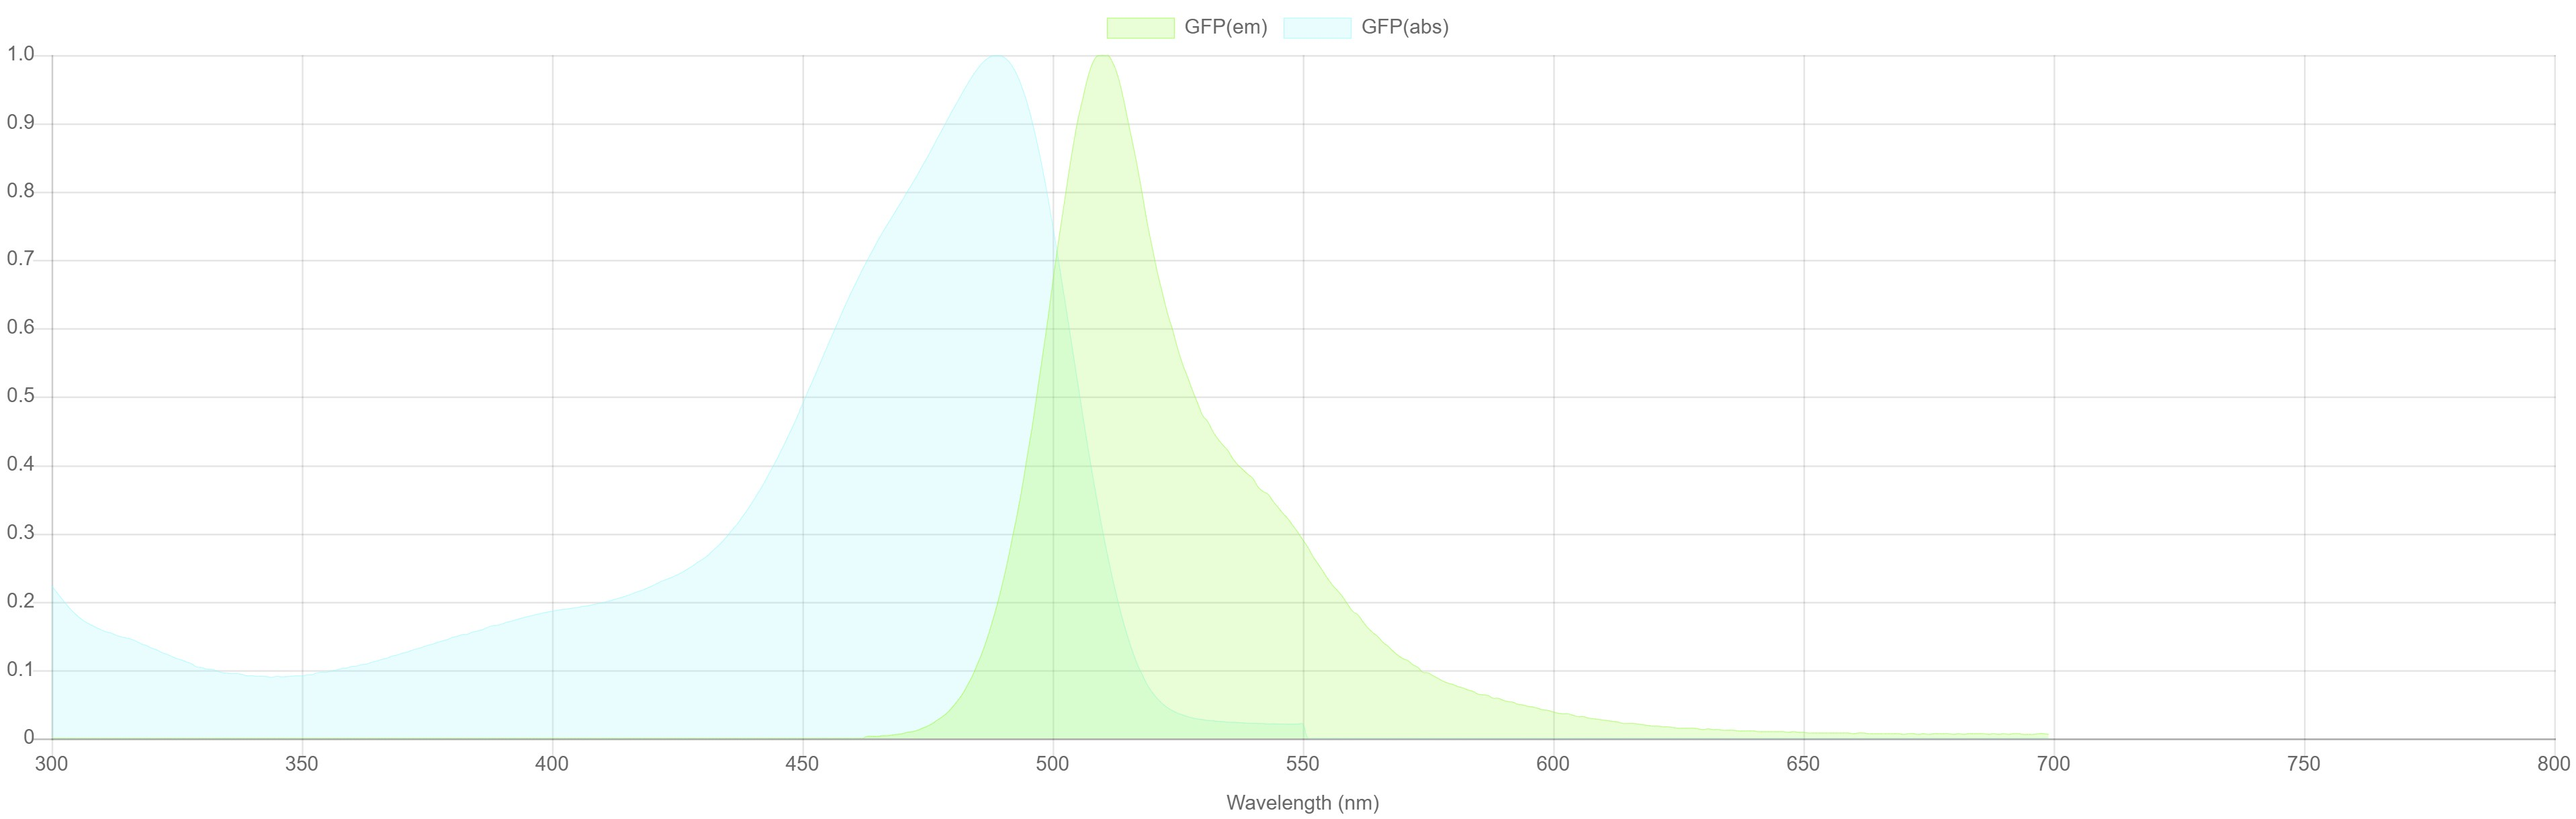
\includegraphics[width=\textwidth]{images/GFP_emission_absorption_spectra.jpg}
	\caption[Example excitation and emission spectra]{Example excitation (blue) 
		and emission (green) spectra for Green Fluorescent Protein. Generated with SpekCheck\cite{phillips2018spekcheck}}
	\label{fig:GFP_emission_absorption_spectra}
\end{sidewaysfigure*}

The first fluorescence microscopes were developed at the beginning of the 20th Century\cite{yuste2005fluorescence,renz2013fluorescence}. The real power of 
fluorescence microscopy came as the specificity of labelling improved. The 
first iteration of this was the development of antibody fluorescent labelling 
which allowed for, among other things, localisation of viral particles in 
biological 
cultures\cite{coons1942demonstration,coons1951fluorescent,weller1954fluorescent}.
The second, and arguably more profound, iteration was the discovery and 
cloning of \textit{Aequorea Victoria} GFP, and the development of chromatic
variants\cite{prasher1992primary,heim1996engineering}. This allowed for 
specific proteins of interest to be individually labelled and for biologists 
to monitor gene-expression\cite{chalfie1994green}. Since then, additional 
properties of fluorescent proteins, such as their conformational changes 
in response to binding events, environmental changes, or enzymatic activity, 
have been utilised to great effect\cite{toseland2013fluorescent}. 
Fluorescence microscopy has allowed biologists to visualise dynamic biological
processes in real time.

\subsection{Resolution}
\label{subsec:resolution}

A fundamental property of all microscopes and microscopy images is that of 
resolution - the minimum separation between two objects where they can still
be determined to be two distinct objects. Consider an optical plane, 
$\textbf{O}$, where a biological specimen is placed - the `sample plane'. Also
consider a separate optical plane, $\textbf{O'}$, where the image of the
specimen is formed - the `image plane'. The microscope, with circular entrance
and exit pupils, maps the field distributions between $\textbf{O}$ and 
$\textbf{O'}$. Figure~\ref{fig:simplified_microscope_layout} shows a schematic
of this simplified system.

\begin{figure}[h]
	\centering
	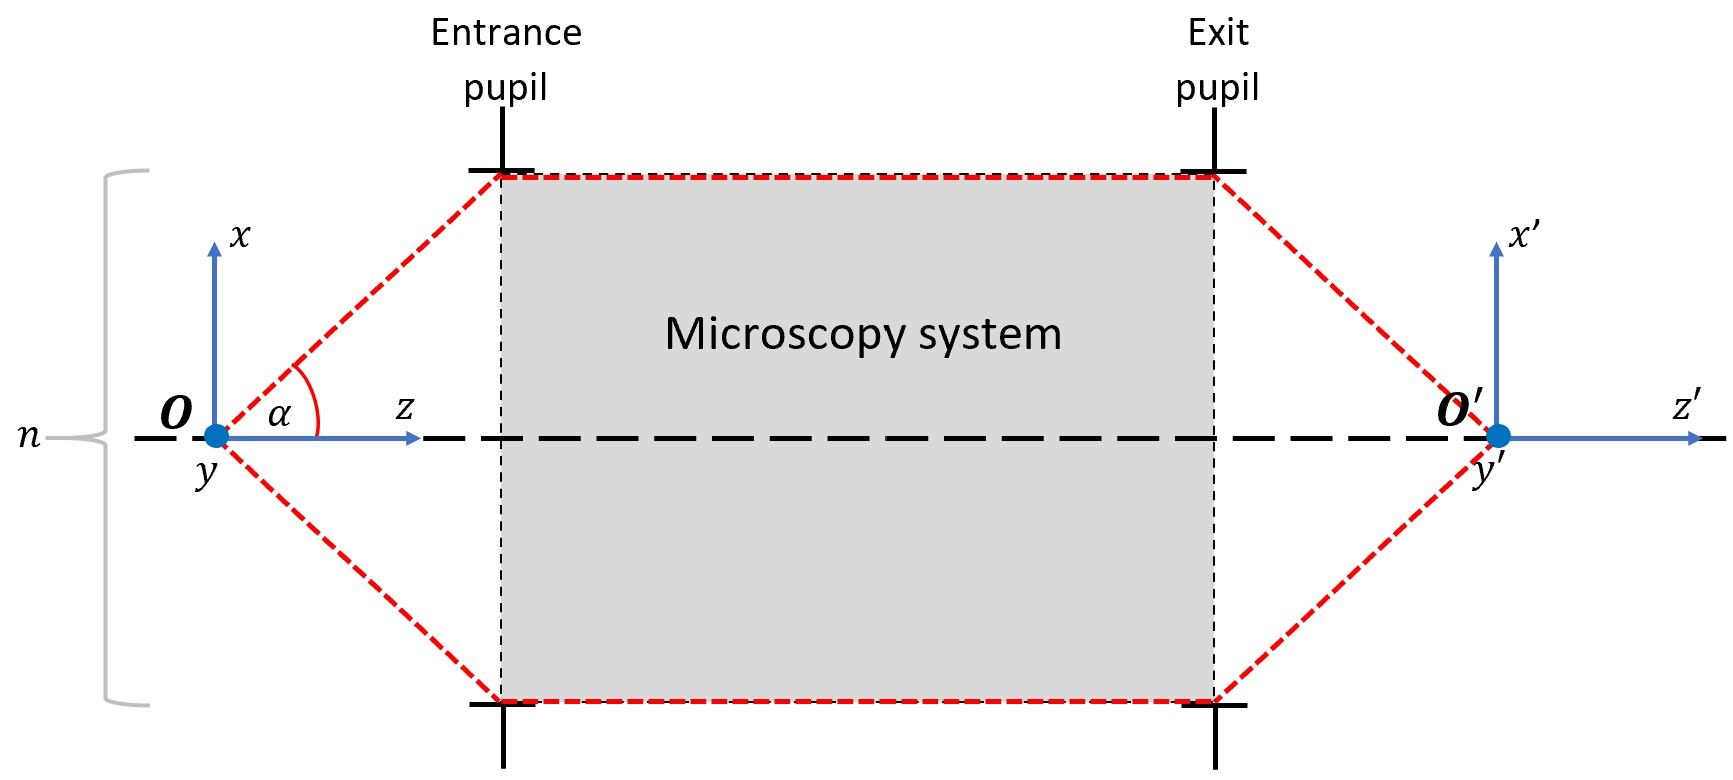
\includegraphics[width=\textwidth]{images/simplified_microscope_layout.jpg}
	\caption[A simplified schematic of a light microscope.]{A simplified 
		schematic of a light microscope. A specimen 
		is placed at the sample plane, $\textbf{O}$, in refractive index, $n$. Light 
		rays emerging from $\textbf{O}$ are collected by the entrance pupil. These 
		rays process through the microscope system before emerging at the exit pupil 
		and being focused at the image plane, $\textbf{O'}$. The light rays which 
		form and angle with the optical axis, $\textbf{OO'}$, of $\alpha$ are called
		marginal rays. Marginal rays are the highest XX diffraction order collectable by
		the entrance pupil XX (NO this is only true is
                transmission. In fl the light isnt diffracted, it is
                just the highest angle of light that can be collected.
                XX) and therefore the microscope system as a whole.}
	\label{fig:simplified_microscope_layout}
\end{figure}

Consider a point source located at $\textbf{O}$ isotopically emitting 
monochromatic light of wavelength $\lambda$. Every ray forms an angle, 
$\theta$, with the optical axis $\textbf{OO'}$. The highest angle collected
by the entrance pupil is $\alpha$. A point source can be considered an 
infinitely narrow aperture and $\alpha$ determines the highest 
diffraction order which the entrance pupil - i.e. the microscope
objective aperture - can collect\cite{davidson2002optical}. Considering this 
and, more generally, the diffraction of light through a circular aperture 
it is possible to obtain that the field intensity at \textbf{O'} is 
proportional to\cite{goodman2005introduction,born2013principles}:

\begin{equation}\label{eq:image_field_insentity}
\mathcal{I}_{w}(v) = \left|\frac{2\mathcal{J}_{1}(v)}{v}\right|^2,
\end{equation}

where $\mathcal{J}_{1}(v)$ is the first-order Bessel function of the first 
kind of the variable $v$\cite{watson1995treatise}. $v$ is the normalised 
lateral co-ordinate given by\cite{wilson1984theory}:

\begin{equation}\label{eq:normalised_lateral}
v = \frac{2\pi}{\lambda}rn\sin(\alpha).
\end{equation}

$r$ is the radial displacement in the image plane $\textbf{O'}$, $r = \sqrt{x'^{2} + y'^{2}}$. 
A useful quantity, and one often cited by microscope objective manufacturers, 
is the numerical aperture, $NA = n\sin(\alpha)$. The Rayleigh criterion 
determines that the limit at which two point objects can be meaningfully 
separated is when the central maxima of one diffraction pattern lies in the
first minimal of the other\cite{rayleigh1874xii,rayleigh1880investigations}. For a first order Bessel 
function, this occurs at $v \approx 1.22\pi$. Therefore, the lateral resolution 
limit, $r_l$ is often quoted as:

\begin{equation}\label{eq:lateral_res}
r_l \approx \frac{1.22\lambda}{2NA}
\end{equation}

otherwise known as the Abbe diffraction limit\cite{abbe1873beitrage}
(XX NO abbe limit is 0.5*lambda/NA. Related but different contrast limitXX). Through
a similar process and considering the field intensity along the $z'$ axis, the
axial resolution, $r_a$, is given as\cite{pawley2006handbook}:

\begin{equation}\label{eq:axial_res}
r_a \approx \frac{2\lambda n}{NA^{2}}.
\end{equation}

Figure~\ref{fig:Airy_ring_2_object_seperation} shows two 
diffraction-limited point objects at variable lateral separations. For 
lateral separations less than $r_{l}$ the field intensities resemble a single 
point source in the image plane. For lateral separation at or above $r_{l}$ 
the intensity contributions from the two objects are distinguishable as 
separate.

\begin{figure}[h]
	\centering
	\begin{subfigure}{0.49\textwidth}
		\centering
		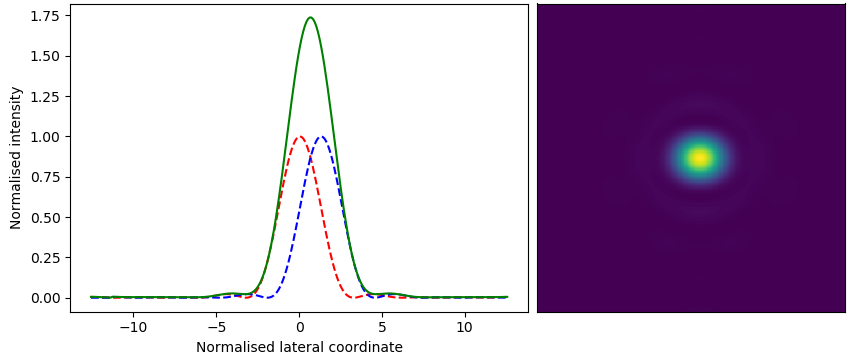
\includegraphics[width=\linewidth]{images/Airy_ring_2_object_seperation_0_5.png}
		\caption{Object separation = $0.41\text{r}_{\text{l}}$}
		\label{fig:Airy_ring_2_object_seperation_0_5}
	\end{subfigure}
	\begin{subfigure}{0.49\textwidth}
		\centering
		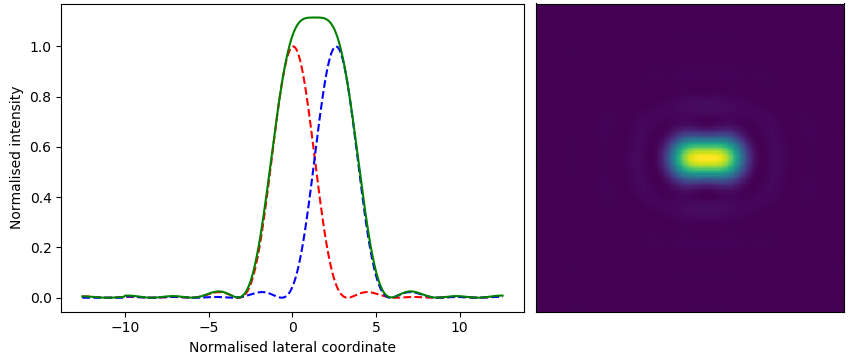
\includegraphics[width=\linewidth]{images/Airy_ring_2_object_seperation_1_0.png}
		\caption{Object separation = $0.82\text{r}_{\text{l}}$}
		\label{fig:Airy_ring_2_object_seperation_1_0}
	\end{subfigure}
	\begin{subfigure}{0.49\textwidth}
		\centering
		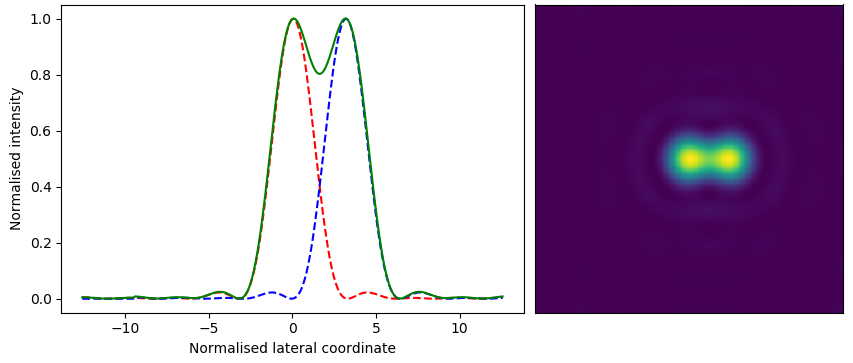
\includegraphics[width=\linewidth]{images/Airy_ring_2_object_seperation_1_22.png}
		\caption{Object separation = $1.0\text{r}_{\text{l}}$}
		\label{fig:Airy_ring_2_object_seperation_1_22}
	\end{subfigure}
	\begin{subfigure}{0.49\textwidth}
		\centering
		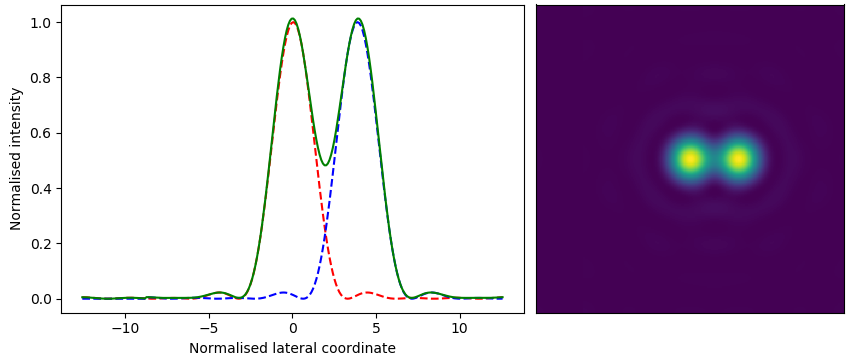
\includegraphics[width=\linewidth]{images/Airy_ring_2_object_seperation_1_5.png}
		\caption{Object separation = $1.23\text{r}_{\text{l}}$}
		\label{fig:Airy_ring_2_object_seperation_1_5}
	\end{subfigure}
	\caption[Illustration of the resolution limit as determined by the Rayleigh
	criterion]{Illustration of the resolution limit as determined by the Rayleigh 
		criterion. Each subfigure shows a line profile and 2D plot of the field 
		intensity distributions of both of the two diffraction limited point 
		objects. For two point objects separated by $< r_{l}$, \textbf{(a)} \& 
		\textbf{(b)}, they are not separable as individual objects. At a 
		separation $\ge r_{l}$, \textbf{(c)} \& \textbf{(d)}, the two point 
		objects are separable.}
	\label{fig:Airy_ring_2_object_seperation}
\end{figure}

Several approximations had to be made to obtain Equations~\ref{eq:lateral_res}
and~\ref{eq:axial_res}. Firstly, the Fraunhofer and paraxial approximations are
assumed to hold\cite{goodman2005introduction}. Obviously, the microscope system
has been greatly simplified to essentially just the entrance and exit pupils. 
More complex but accurate models for modern microscopy set-ups have been 
demonstrated\cite{torok2007optical, foreman2011computational}. Finally, this
idealised system only considers the shape of the apertures - i.e. the entrance
and exit pupils - and the wavelength of light. If one were to observe objects 
such as these, with these field distributions corresponding to well-specified
models, there would be no resolution limit at all\cite{den1997resolution}. In 
practice, the field distributions of objects are not precisely known, therefore
determining the location of the first minima is not as simple as it has been 
presented here. The first minima may not even be radially symmetric. 

Furthermore, the `true' resolution achievable by a microscopy system is 
affected by other factors such as the signal-to-noise ratio of an
image (XX in fact the difefrence bewteen for instance the abbe and
reyleigh limits can be atributed to s:n. Reighley assumes a ~25\% dip
between peaks Abbe is much lessXX), 
coherence conditions of illumination, apodization, discretisation errors for 
digital cameras, to name a few\cite{den1997resolution}. There have been 
attempts to develop alternative resolution measurements for point 
objects\cite{ram2006beyond}. Unfortunately, the actual resolution achieved in 
biological samples varies across the image plane, determined by factors such 
as the labelling density of the underlying biological 
specimen\cite{culley2017nanoj}. The `true' resolution of a system for a given 
sample is therefore a quantity which is impossible to determine analytically. 
The ideal lateral and axial resolutions in Equations~\ref{eq:lateral_res} 
and~\ref{eq:axial_res} are nonetheless useful quantities as the theoretical, 
ideal resolution limit of a microscopy system.

Returning to the concept of a point object as an infinitely narrow aperture allows 
for a more complete understanding of the resolution limit. A spatially structured 
object can be described by a superposition of spatial frequencies in the same 
manner in which a temporally structured object can be described by a superposition 
of temporal frequencies, which is the basis for Fourier 
optics\cite{goodman2005introduction}. A point object can be described as a Dirac
delta function, the Fourier transform of which is a uniform distribution across all
spatial frequencies. The addition of an aperture, such as a microscope objective, 
effectively imposes a low-pass filter on the spatial frequency domain. 
Figure~\ref{fig:WF_OTF} shows the projection of the observable region onto the 
lateral spatial frequency plane $k_{x}k_{y}$ i.e. the low-pass filter. The radius of
this low-pass filter is: 

\begin{equation}\label{eq:lateral_spatial_freq_res}
\omega_{l} = \frac{1}{r_{l}},
\end{equation}

where $r_{l}$ is the lateral resolution limit. The bounds of the observable region 
in $k_{z}$ differs since the intensity spectrum - the power spectrum of the 
field intensity - in $k_{z}$ is independent of the object nature and the point
spread function\cite{frieden1967optical}. The bounds of the observable region in
$k_{z}$ can be shown to be:

\begin{equation}\label{eq:observable_region_kz}
k_{z} = \pm\frac{\left\|\textbf{k}_{xy}\right\|}{2\lambda_{k}}(\omega_{l} - \left\|\textbf{k}_{xy}\right\|),
\end{equation}

for $\left\|\textbf{k}_{xy}\right\| \le \omega_{l}$ where 
$\left\|\textbf{k}_{xy}\right\|$ is the length of the vector denoting the 
lateral spatial frequencies, $(k_{x},k_{y})$ and $\lambda_{k} = 
\frac{2\pi}{\lambda}$\cite{frieden1967optical}. Figure~\ref{fig:WF_OTF_xz} shows 
the projection of the observable region onto the axial spatial frequency plane 
$k_{x}k_{z}$. The maximum extension of this observable region, $k_{a}$, is given 
by:

\begin{equation}\label{eq:axial_observable_max_k}
\omega_{a} = \frac{\omega_{l}^{2}}{8\lambda_{k}},
\end{equation}

From Equation~\ref{eq:observable_region_kz}, the observable
region in $k_{z}$ is bandpass limited at both high and low spatial frequencies.
This results in the ``missing cone'' phenomenon which limits the axial spatial 
frequencies which are able to be collected, in turn limiting the axial 
resolution\cite{behan2009three,arnison20023d}. This, coupled with the fact that
for all practical cases $k_{a} \ll k_{l}$, explains why the axial resolution is
always worse than the lateral resolution of a system. Figure~\ref{fig:WF_OTF} 
shows the complete 3D observable region, obtained by rotating 
Figure~\ref{fig:WF_OTF_xz} around the $k_{z}$ axis. Only spatial frequencies
within this observable region contribute to the observed sample structure.
The observable region can be described as:

\begin{equation}\label{eq:observable region}
O_{0}(\textbf{k}) = 
\begin{cases}
1, & if~ \left\|\textbf{k}_{xy}\right\| < \omega_{l} ~and~ \left\|k_{z}\right\| < \frac{\left\|\textbf{k}_{xy}\right\|}{2\lambda_{k}}(\omega_{l} - \left\|\textbf{k}_{xy}\right\|)\\
0, & otherwise\\
\end{cases}.
\end{equation}

\begin{figure}[h]
	\centering
	\begin{subfigure}[t]{0.23\textwidth}
		\centering
		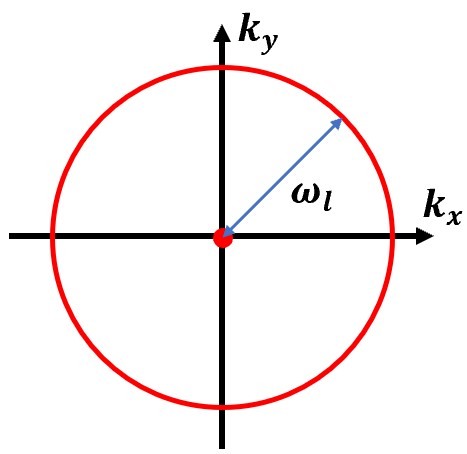
\includegraphics[width=\linewidth]{images/3D_SIM_OTF_no_angle_2D_plot_xy_k_l.jpg}
		\caption{}
		\label{fig:WF_OTF_xy}
	\end{subfigure}
	\begin{subfigure}[t]{0.4\textwidth}
		\centering
		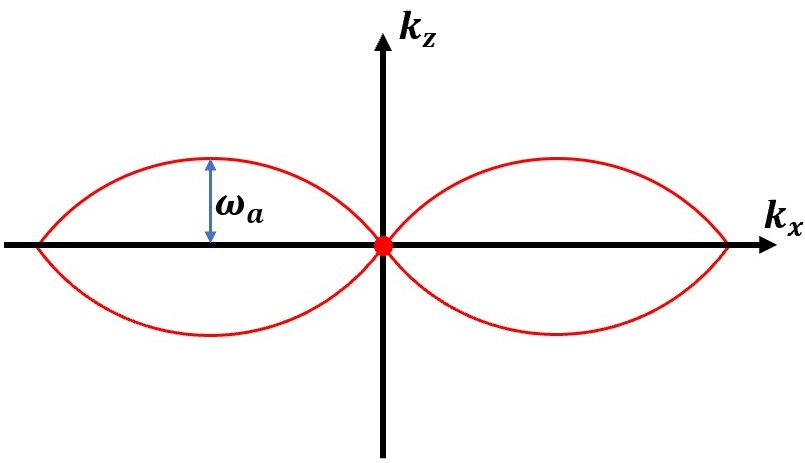
\includegraphics[width=\linewidth]{images/3D_SIM_OTF_no_angle_2D_plot_xz_k_a.jpg}
		\caption{}
		\label{fig:WF_OTF_xz}
	\end{subfigure}
	\begin{subfigure}[t]{0.27\textwidth}
		\centering
		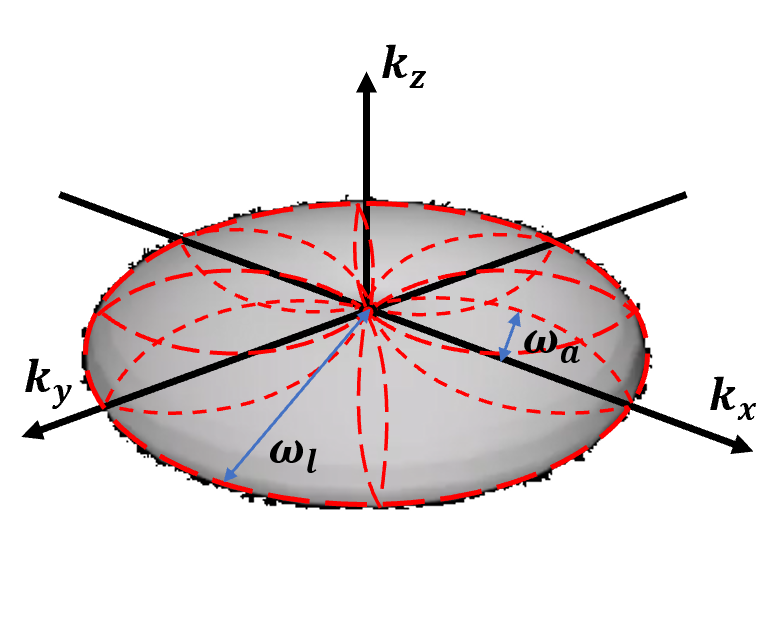
\includegraphics[width=\linewidth]{images/3D_SIM_OTF_no_angle_axis.png}
		\caption{}
		\label{fig:WF_OTF}
	\end{subfigure}
	\caption[Widefield observable region visualisation]{Widefield observable 
		region visualisation. \textbf{(a)} The projection of the observable 
		region onto the $k_{x}k_{y}$ plane. \textbf{(b)} The projection of 
		the observable region onto the $k_{x}k_{z}$ plane. \textbf{(c)} The 
		full observable region for a conventional widefield microscope in 
		reciprocal space.}
	\label{fig:widefield_OTF_visualisation}
\end{figure}

\section{Super-resolution Microscopy}
\label{sec:super_res}

For some time, the diffraction limit represented a kind of practical 
resolution asymptote - a point to be approached but never reached. Two
`gold standard' techniques for optical bioimaging emerged thanks to their
ease of implementation and how close they were able to get to the diffraction
limit; deconvolution\cite{agard1983three, wallace2001workingperson} and
confocal laser scanning microscopy\cite{sheppard1981theory,minsky1988memoir}. 
Nonetheless, the instant one defines a limit it is practically human nature 
to attempt to surpass it. Therefore, a number of `super-resolution' techniques
have emerged capable of surpassing even the ideal diffraction limit. These
can be broadly divided into two categories: near-field and far-field methods.
Near-field methods, whilst capable of achieving resolutions of $\sim 20 nm$,
are only suitable for surface structure imaging\cite{schermelleh2010guide}. 
Far-field techniques fall into 4 broad techniques: structured illumination
microscopy (SIM), stimulated emission depletion (STED) microscopy, 
single-molecule localisation microscopy (SMLM) and interferometric-based 
techniques. There are some implementations which combine several 
techniques. Each super-resolution technique has benefits and drawbacks which 
need to be considered when employing them including; the resolution 
(laterally and axially) required and the resolution achievable with each 
technique, acquisition speed, photodamage incurred, depth of imaging and 
multi-colour capability\cite{hell20152015,schermelleh2019super} Although it 
has a modest resolution improvement, SIM is the most widely accepted 
super-resolution technique for biology thanks to its multi-colour capability,
high temporal resolution and low photodamage impact\cite{leung2011review}.

\subsection{Structured Illumination Microscopy}
\label{subsec:SIM}

There are a number of microscopy techniques which fall under the structured
illumination microscopy umbrella: Re-scan\cite{de2013re}, 
Airyscan\cite{huff2015airyscan}, iSIM\cite{york2013instant,curd2015construction},
and SIMFlux\cite{cnossen2020localization} to name a few. Whilst all these can be 
considered `structured illumination' techniques since they do rely on spatially 
structured excitation light, for the duration of this thesis the term 
`structured illumination microscopy' or SIM refers to the form of 
interference-based microscopy pioneered by Mats 
Gustafsson\cite{gustafsson1999extended,gustafsson2000surpassing,gustafsson2008three}
(XX probably should ref the early Heizmann and Cremer paper(s)XX https://www.spiedigitallibrary.org/conference-proceedings-of-spie/3568/0000/Laterally-modulated-excitation-microscopy--improvement-of-resolution-by-using/10.1117/12.336833.short?SSO=1).
This implementation of SIM is best understood through the moir\'{e} effect.
Two patterns, such as those shown in Figure~\ref{fig:fringes_1} and 
\ref{fig:fringes_1}, which are multiplicatively superimposed on one another
will produce a beat pattern - moir\'{e} fringes - such as those shown in
Figure~\ref{fig:fringes_moire}. Using the convolution theorem, the Fourier
transform of this superposition is equivalent to the convolution of the 
Fourier transforms of the two original patterns\cite{mcgillem1991continuous},
as shown in Figures~\ref{fig:fringes_1_ft}-\ref{fig:fringes_moire_ft}. 

\begin{figure}[h]
	\centering
	\begin{subfigure}[t]{0.3\textwidth}
		\centering
		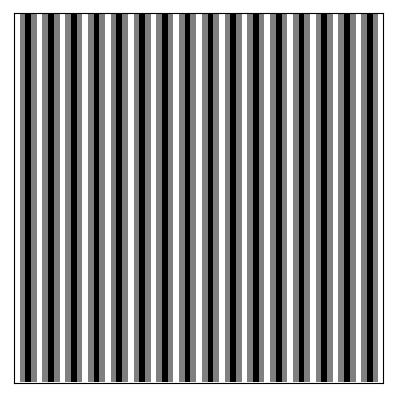
\includegraphics[width=\linewidth]{images/fringes_1_kx_16_ky_0.png}
		\caption{}
		\label{fig:fringes_1}
	\end{subfigure}
	\begin{subfigure}[t]{0.3\textwidth}
		\centering
		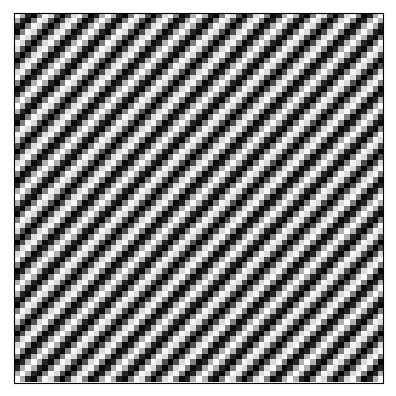
\includegraphics[width=\linewidth]{images/fringes_2_kx_12_ky_12.png}
		\caption{}
		\label{fig:fringes_2}
	\end{subfigure}
	\begin{subfigure}[t]{0.3\textwidth}
		\centering
		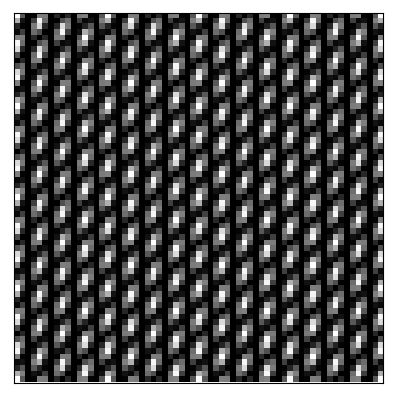
\includegraphics[width=\linewidth]{images/fringes_moire_kx_16_and_12_ky_0_and_12.png}
		\caption{}
		\label{fig:fringes_moire}
	\end{subfigure}
	
	\begin{subfigure}[t]{0.3\textwidth}
		\centering
		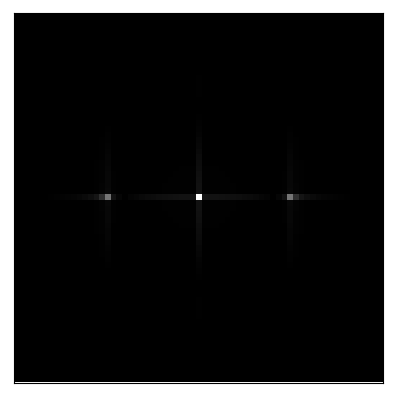
\includegraphics[width=\linewidth]{images/fringes_1_ft_kx_16_ky_0.png}
		\caption{}
		\label{fig:fringes_1_ft}
	\end{subfigure}
	\begin{subfigure}[t]{0.3\textwidth}
		\centering
		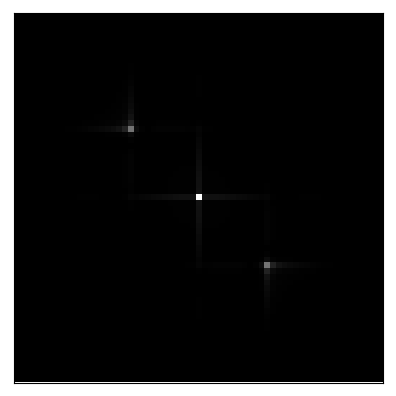
\includegraphics[width=\linewidth]{images/fringes_2_ft_kx_12_ky_12.png}
		\caption{}
		\label{fig:fringes_2_ft}
	\end{subfigure}
	\begin{subfigure}[t]{0.3\textwidth}
		\centering
		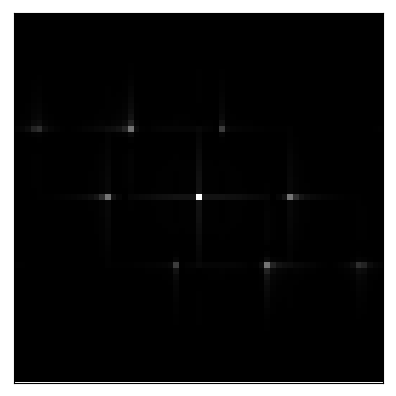
\includegraphics[width=\linewidth]{images/fringes_moire_ft_kx_16_and_12_ky_0_and_12.png}
		\caption{}
		\label{fig:fringes_moire_ft}
	\end{subfigure}
	\caption[Visualisation of moir\'{e} fringes]{Visualisation of moir\'{e} 
		fringes. \textbf{(a)}-\textbf{(b)} shows two spatially structured images. 
		\textbf{(c)} shows the resultant moir\'{e} fringes arising from the 
		interference of \textbf{(a)} and \textbf{(b)}. \textbf{(d)}-\textbf{(f)} 
		shows the respective Fourier transforms of \textbf{(a)}-\textbf{(c)}. 
		Note that \textbf{(f)} is a convolution of \textbf{(d)} and \textbf{(e)}}
	\label{fig:moire_visualisation}
\end{figure}

For SIM, one of the patterns is the underlying biological structure - or more 
specifically the spatial distribution of fluorophores - and the other is the 
spatially structured excitation illumination. The moir\'{e} fringes arising 
from the superposition of these two structures can be coarser than either of 
the original patterns, meaning that moir\'{e} fringes arising from the 
superposition of biological structures beyond the resolution limit of the 
microscope and a known illumination pattern can be observed. These moir\'{e} 
fringes contain information about these super-resolution structures and the
super-resolution information can be extracted from the moir\'{e} fringes, 
effectively extending the observable region of a microscope beyond the 
diffraction limit\cite{gustafsson2000surpassing}.

A single fluorescent image, $F(\textbf{r})$, is defined by:

\begin{equation}\label{eq:fluorescent_image}
\begin{split}
F(\textbf{r}) &= (E \circledast H)(\textbf{r})\\
F(\textbf{r}) &= [D(\textbf{r})I(\textbf{r})] \circledast H(\textbf{r}),\\
\end{split},
\end{equation}

Where $D(\textbf{r})$ is the sample fluorescence distribution, 
$I(\textbf{r})$ is the illumination pattern, $E(\textbf{r})$ is the resultant 
emission signal, $H(\textbf{r})$ is the system point spread function (PSF) 
and $\circledast$ represents the convolution operation. Applying the 
convolution theorem and a Fourier transform yield:

\begin{equation}\label{eq:SIM_fluorescent_image_fourier}
\begin{split}
\mathcal{F}\left[F(\textbf{r})\right] &= \mathcal{F}\left[\left[D(\textbf{r})I(\textbf{r})\right] \circledast H(\textbf{r})\right]\\
\tilde{F}(\textbf{k}) &= \left[\tilde{D}(\textbf{k})\circledast \tilde{I}(\textbf{k})\right] \tilde{H}(\textbf{k})\\
\tilde{F}(\textbf{k}) &= \left[\tilde{D}(\textbf{k})\circledast \tilde{I}(\textbf{k})\right] O(\textbf{k}),\\
\end{split},
\end{equation}

Where $\sim$ indicated the Fourier transform of the respective real-space
functions. $O(\textbf{k}) = \tilde{H}(\textbf{k})$ is the optical transfer
function (OTF) of the imaging system. The complex values of $O(\textbf{k})$
describe the attenuation of the spatial frequencies within the observable 
region described by Equation~\ref{eq:observable region}. For uniform 
illumination - i.e. widefield imaging - $\tilde{I}(\textbf{k}) = \delta(0)$ 
where $\delta$ is the Dirac delta function, and therefore only the spatial 
frequencies within the observable region contribute to the image formation as 
previously noted.  However, if $I(\textbf{r})$ is spatially structured then 
the convolution $\tilde{D}(\textbf{k})\circledast \tilde{I}(\textbf{k})$ is 
non-local and the  data within the observable region contains contributions 
from spatial frequencies which are normally outside the observable region.

For a general illumination pattern, extracting these super-resolution 
contributions from the diffraction limited contributions is non-trivial.
However, imposing some conditions on the illumination structure simplifies
this process\cite{gustafsson2008three}. Firstly, the illumination pattern 
should consist of the sum of a finite number, $m$, of components and these
components should be separable into axial and lateral components. The 
illumination pattern, $I(\textbf{r}_{xy},z)$, is therefore:

\begin{equation}\label{eq:illumination_components}
I(\textbf{r}_{xy},z) = \sum\limits_{m}{I_{m}(z)J_{m}(\textbf{r}_{xy})},
\end{equation}

where $\textbf{r}_{xy}$ the vector denoting the lateral coordinates, $(x,y)$.
Secondly, the lateral functions, $J_{m}(\textbf{r}_{xy})$, should be purely
harmonic functions meaning they contain only one spatial frequency. Note that 
the lateral functions, $J_{m}$, should not be confused with the first-order 
Bessel functions, $\mathcal{J}_{1}$ from before. Finally, the axial 
functions, $I_{m}(z)$, should either: 

\begin{enumerate}
	\item also be purely harmonic functions.
	\item in instances where 3D data is acquired as a series of 2D images with 
	different focus - as in microscopy - the illumination pattern is maintained 
	fixed relative to the focal plane of the microscope and not relative to the
	objecting being imaged.
\end{enumerate}

The first and third conditions allow Equation~\ref{eq:fluorescent_image} to be
written as:

\begin{equation}\label{eq:fluorescent_image_conditions}
\begin{split}
F(\textbf{r}) &= [D(\textbf{r})I(\textbf{r})] \circledast H(\textbf{r})\\
F(\textbf{r}) &= \sum\limits_{m}{\int H(\textbf{r}-\textbf{r}'))I_{m}(z - z')D(\textbf{r}')J_{m}(\textbf{r}'_{xy})}d\textbf{r}'\\
F(\textbf{r}) &= \sum\limits_{m}{\left[HI_{m}\circledast DJ_{m}\right](\textbf{r})}\\
\end{split},
\end{equation}

where $\textbf{r}'$ denotes the sample reference from, $\textbf{r}$ denotes
the data-set reference frame and $\textbf{r} - \textbf{r}'$ denotes the 
reference frame of the objective. Taking the Fourier transform of the 
$m$-th term, $F_{m}(\textbf{r})$, yields:

\begin{equation}\label{eq:fluorescent_image_mth_ft}
\tilde{F}_{m}(\textbf{k}) = \tilde{O}_{m}\left[\tilde{D}(\textbf{k}) \circledast \tilde{J}_{m}(\textbf{k}_{xy})\right],
\end{equation}

where $\tilde{O}_{m} = O \circledast \tilde{I}_{m} = \mathcal{F}[HI_{m}]$.
Here the second condition of the lateral functions being purely harmonic allows
$J_{m}(\textbf{r}_{xy})$ to be written as:

\begin{equation}\label{eq:lateral_illumination}
J_{m}(\textbf{r}_{xy}) = e^{i\left(2\pi\textbf{p}_m\cdot\textbf{r}_{xy} + \phi_{m}\right)},
\end{equation}

\begin{equation}\label{eq:lateral_illumination_ft}
\Rightarrow \tilde{J}_{m}(\textbf{k}_{xy}) = \delta\left(\textbf{k}_{xy} - \textbf{p}_m\right)e^{i\phi_{m}},
\end{equation}

Substituting Equation~\ref{eq:lateral_illumination_ft} into 
Equation~\ref{eq:fluorescent_image_mth_ft} and summing over all $m$ components,
the observed data can be written as:

\begin{equation}\label{eq:single_SIM_image}
\tilde{F}(\textbf{k}) = \sum\limits_{m}{\tilde{O}_{m}(\textbf{k})e^{i\phi_{m}}\tilde{D}\left(\textbf{k} - \textbf{p}_m\right)}.
\end{equation}

Therefore, each image is a sum of a finite number, $N$, copies of the object 
information, $\tilde{D}$, each shifted laterally in reciprocal space by 
$\textbf{p}_{m}$, filtered by the OTF, $O$, and phase shifted by $\phi_{m}$.
Acquiring $N$ images with different values of $\phi_{m}$ gives a system of 
linear equations with as many equations as unknowns. The frequency components
can therefore be separated by applying an $N\times N$ separation matrix. The 
values of $\phi_{m}$ are generally chosen to be evenly spaced between 
$[0,2\pi]$ radians to ensure a well-conditioned separation 
matrix\cite{gustafsson2008three}.

Considering the practical implications further simplifies the situation. 
Firstly, the intensity distribution of light is a real-valued function and
therefore the exponentials in Equation~\ref{eq:lateral_illumination_ft} must
occur in pairs with $\pm\textbf{p}_{m}$. Since the Fourier transform of a 
real-valued function has the symmetry property $\tilde{a}(-\textbf{k}) = 
\bar{\tilde{a}}(\textbf{k})$ only one component need be calculated and the
other can be determined by symmetry. Secondly, if the $\textbf{p}_{m}$ are
chosen such that they are all either the fundamental frequency or higher 
harmonics of the same frequency then $\textbf{p}_{m} = m\textbf{p}$ where
$\textbf{p}$ is the fundamental frequency. Furthermore, if the phases are 
chosen such that $\phi_{m} = m\phi$. Taking these effects into account, 
Equation~\ref{eq:single_SIM_image} becomes:

\begin{equation}\label{eq:single_SIM_image_simple}
\tilde{F}(\textbf{k}) = \sum\limits_{m}{\tilde{O}_{m}(\textbf{k})e^{im\phi}\tilde{D}\left(\textbf{k} - m\textbf{p}\right)}.
\end{equation}

Since $O_{m}$ and $\textbf{p}_{m}$ are known, the information components
can be separated and moved by $\textbf{p}_{m}$ back to their correct 
position in reciprocal space, combined to a single extended resolution
spatial frequency dataset, and finally Fourier transformed back into a 
single super-resolution image.  From Equation~\ref{eq:single_SIM_image} 
it is clear that this image is equivalent to an image taken with an 
observable region equal to the convolution of the original system OTF, 
$O$, and the illumination structure Fourier transform, $\tilde{I}$. 

Consider an illumination pattern formed by the interference of two beams 
of light such that $I(\textbf{r}) \propto 1 + \cos(\textbf{r}\cdot
\textbf{p} + \phi)$. Figure~\ref{fig:amplitude_wave_vectors_2D} shows 
the amplitude wave vectors for these beams, both with the same length 
$\frac{1}{\lambda_{ex}}$ where $\lambda_{ex}$ is the wavelength of the 
excitation illumination light. The angle between the two beams determines 
the position of $\textbf{p}$. If $\textbf{p}$ is chosen to be close to 
$k_{l}$ then the spatial frequency components are close to the bounds 
of the observable region, as shown in 
Figure~\ref{fig:2D_SIM_OTF_beam_pos_w_vectors}. The convolution of this 
illumination pattern with the system OTF is shown in 
Figure~\ref{fig:2D_SIM_OTF_1_angle}. The projection of this extended 
observable region on the $k_{x}k_{z}$ plane is shown in 
Figure~\ref{fig:2D_SIM_OTF_1_angle_plot_xz}. The observable region
is laterally extended by a factor, $\alpha_{l}$, given by:

\begin{equation}\label{eq:lateral_res_extension_factor}
\alpha_{l} = \frac{\left(\frac{1}{\lambda_{ex}} + \frac{1}{\lambda_{em}}\right)}{\frac{1}{\lambda_{em}}} = 1 + \frac{\lambda_{em}}{\lambda_{ex}},
\end{equation}

where $\lambda_{ex}$ and $\lambda_{em}$ are the excitation and emission
wavelengths respectively.  However, this extension factor only applied in 
the direction $\overrightarrow{\textbf{p}}$. To achieve isotropic 
resolution enhancement, a number of pattern directions are required. 
Rotating the illumination pattern through the three stripe angles shown 
in Figure~\ref{fig:3D_SIM_OTF_stripe_angles} yields the close to isoptropic extended 
observable region in Figure~\ref{fig:2D_SIM_OTF_all_2D_angles}, the 
projection of which in the $k_{x}k_{y}$ plane is shown in
Figure~\ref{fig:3D_SIM_OTF_xy_expansion_w_double_rad_filled}. 

\begin{figure*}
	\centering
	\begin{subfigure}[t]{0.25\textwidth}
		\centering
		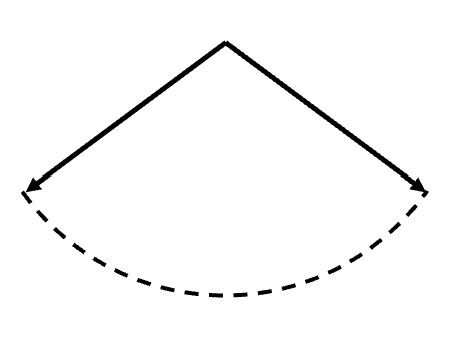
\includegraphics[width=\linewidth]{images/amplitude_wave_vectors_2D.jpg}
		\caption{}
		\label{fig:amplitude_wave_vectors_2D}
	\end{subfigure}
	\begin{subfigure}[t]{0.265\textwidth}
		\centering
		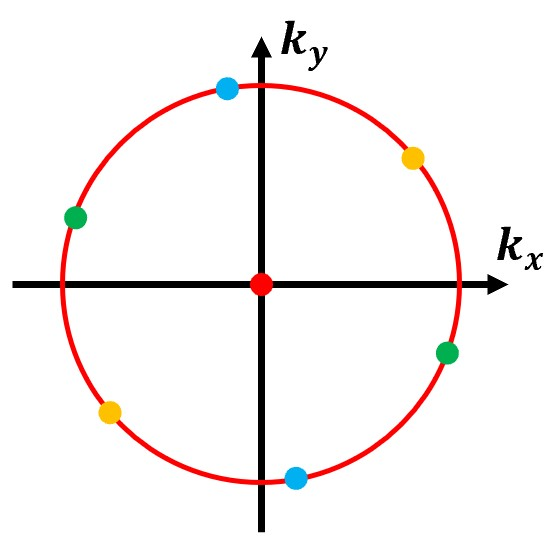
\includegraphics[width=\linewidth]{images/3D_SIM_OTF_stripe_angles.jpg}
		\caption{}
		\label{fig:3D_SIM_OTF_stripe_angles}
	\end{subfigure}
	\begin{subfigure}[t]{0.45\textwidth}
		\centering
		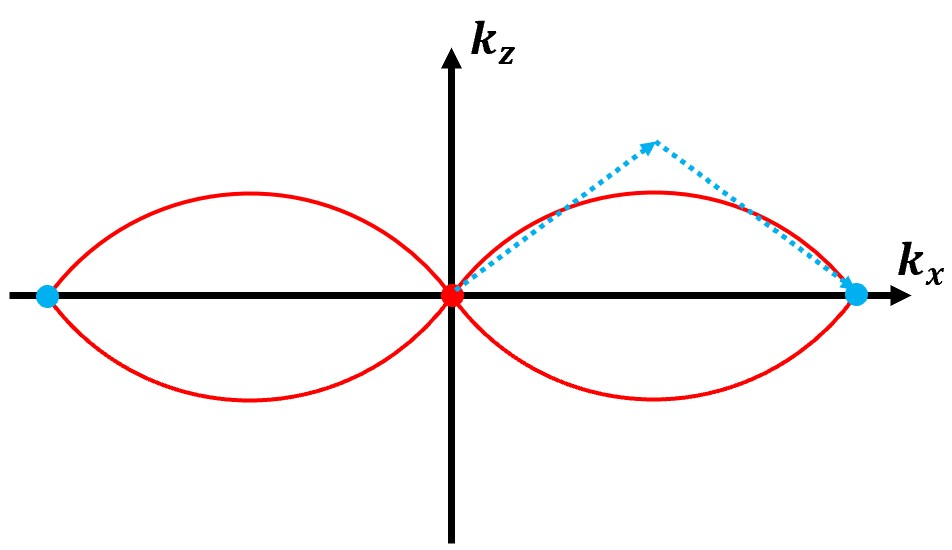
\includegraphics[width=\linewidth]{images/2D_SIM_OTF_beam_pos_w_vectors.jpg}
		\caption{}
		\label{fig:2D_SIM_OTF_beam_pos_w_vectors}
	\end{subfigure}
	
	\begin{subfigure}[t]{0.35\textwidth}
		\centering
		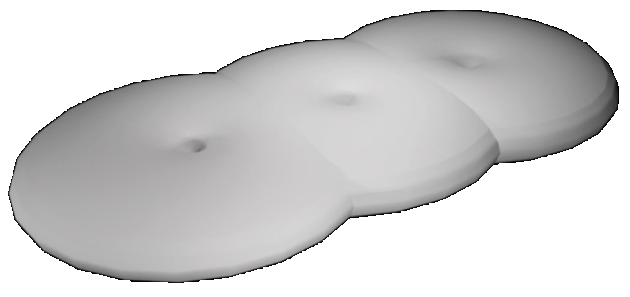
\includegraphics[width=\linewidth]{images/3D_SIM_OTF_1_angle.png}
		\caption{}
		\label{fig:2D_SIM_OTF_1_angle}
	\end{subfigure}
	\begin{subfigure}[t]{0.6\textwidth}
		\centering
		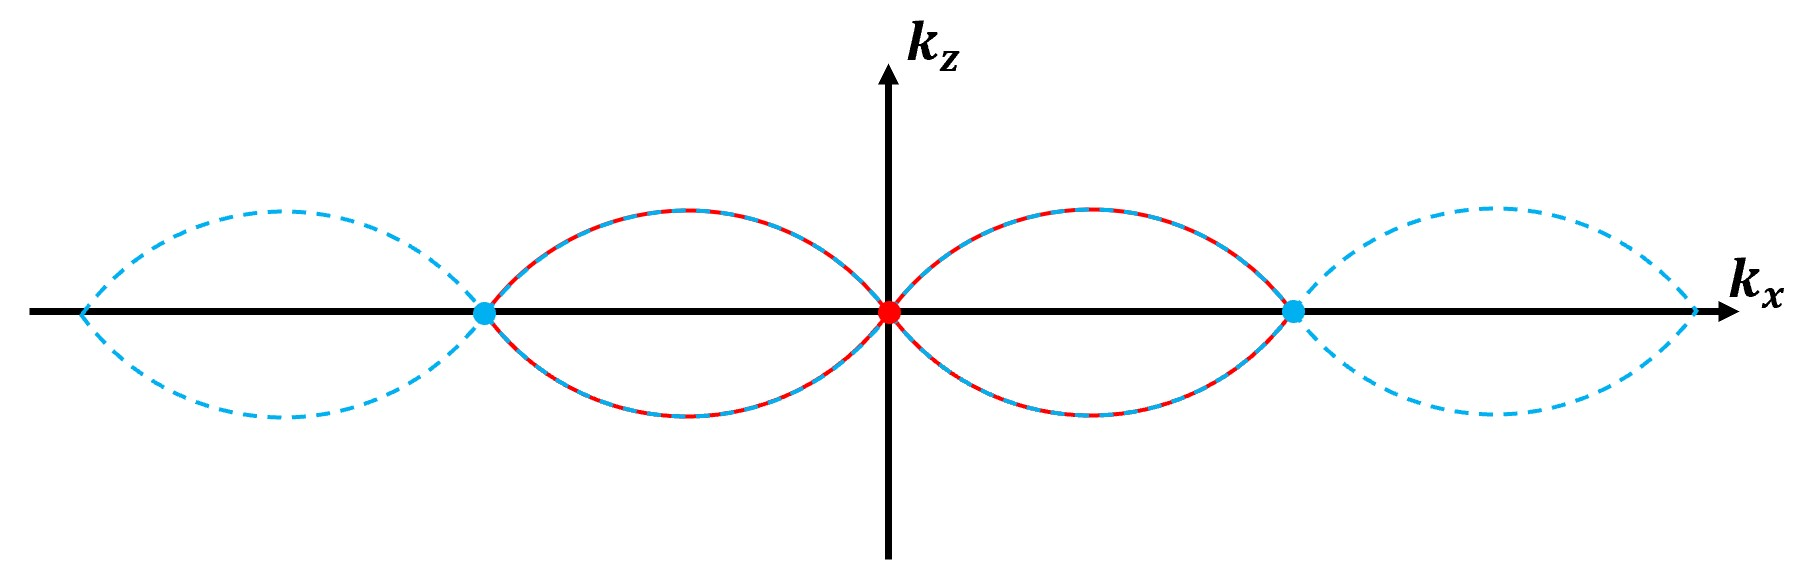
\includegraphics[width=\linewidth]{images/2D_SIM_OTF_1_angle_plot_xz.jpg}
		\caption{}
		\label{fig:2D_SIM_OTF_1_angle_plot_xz}
	\end{subfigure}
	
	\begin{subfigure}[t]{0.4\textwidth}
		\centering
		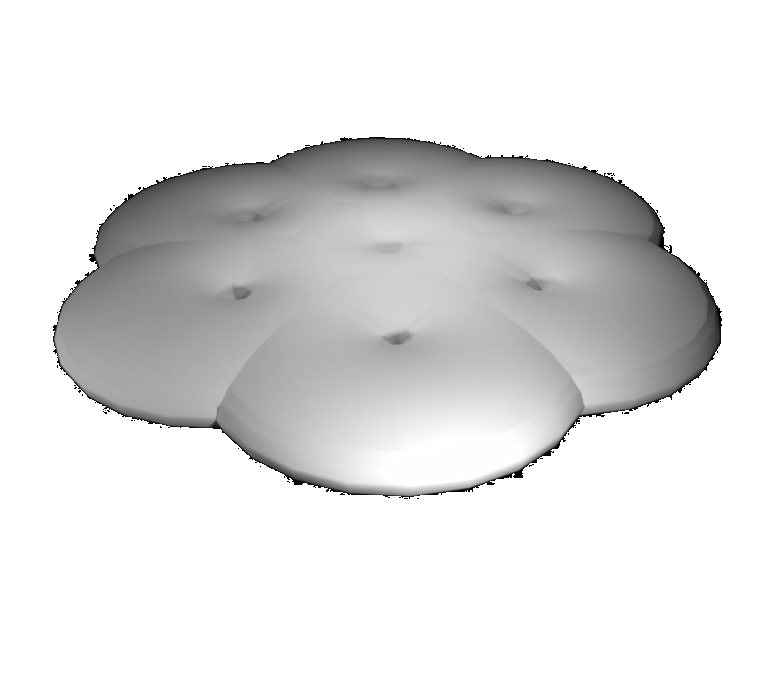
\includegraphics[width=\linewidth]{images/2D_SIM_OTF_all_2D_angles.png}
		\caption{}
		\label{fig:2D_SIM_OTF_all_2D_angles}
	\end{subfigure}
	\begin{subfigure}[t]{0.5\textwidth}
		\centering
		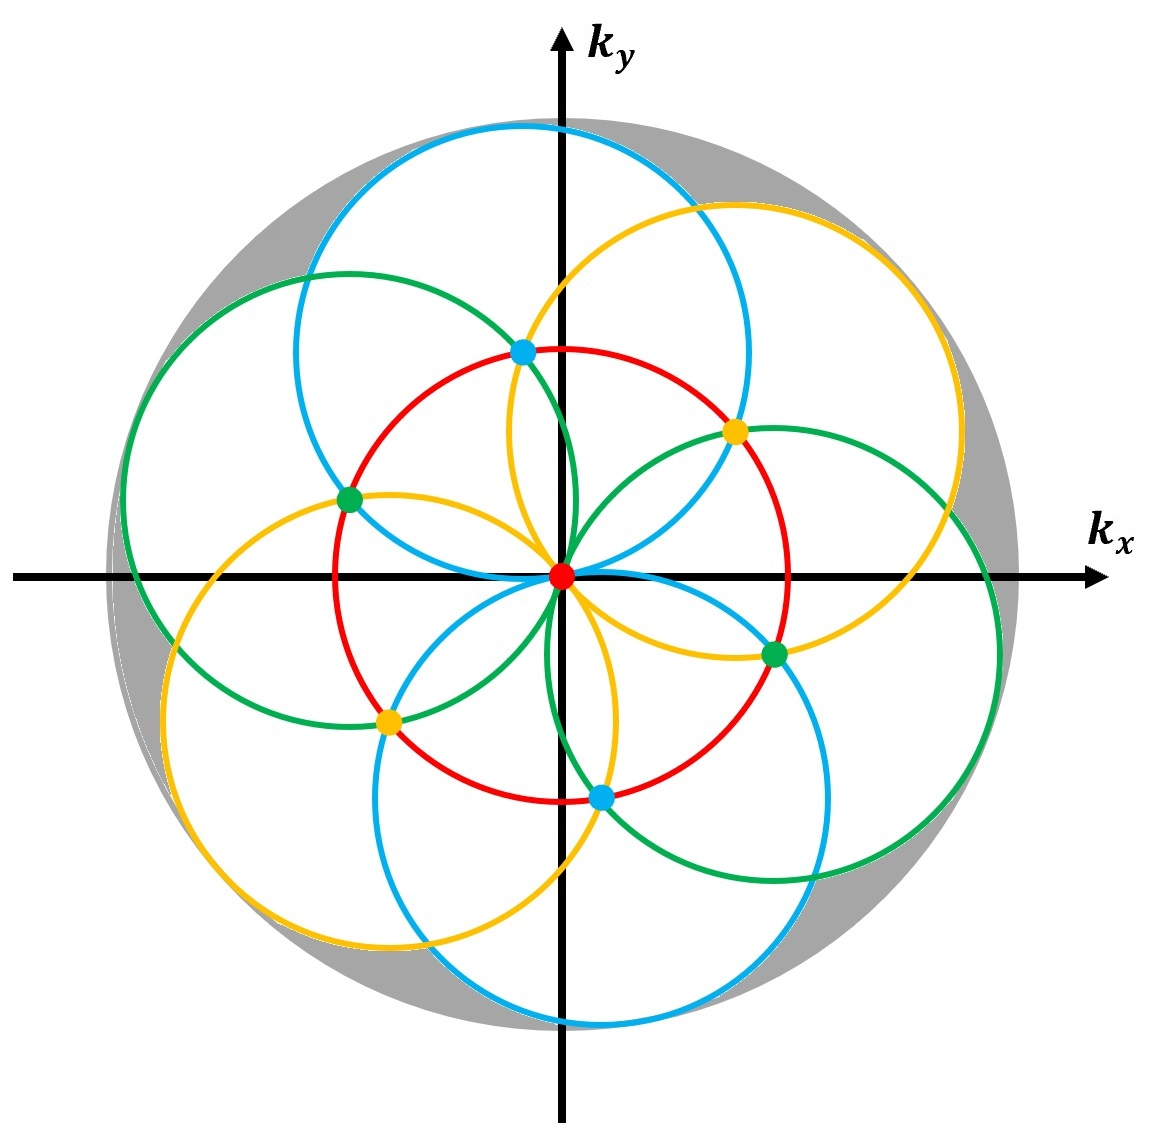
\includegraphics[width=\linewidth]{images/3D_SIM_OTF_xy_expansion_w_double_rad_filled.jpg}
		\caption{}
		\label{fig:3D_SIM_OTF_xy_expansion_w_double_rad_filled}
	\end{subfigure}
	\caption[Resolution enhancement with 2D SIM imaging]{Resolution enhancement 
		with 2D SIM imaging. \textbf{(a)} The amplitude wave vectors 
		corresponding to the 2 illumination beams. Both vectors have the 
		same magnitude, $\frac{1}{\lambda}$ \textbf{(b)} The projection of the 
		observable region onto the $k_{x}k_{y}$ plane with the stripe angles 
		shown \textbf{(c)} The projection of the observable region onto the 
		$k_{x}k_{z}$ plane with the spatial frequency component locations for
		two-beam interference pattern shown. \textbf{(d)} The full observable region 
		extension for one angle in reciprocal space. \textbf{(e)} The projection 
		of the extended observable region in \textbf{(d)} onto the $k_{x}k_{z}$ 
		plane. \textbf{(f)} The full observable region extension for all three angles in 
		reciprocal space. \textbf{(g)} The projection of the extended observable 
		region in \textbf{(f)} onto the $k_{x}k_{y}$ plane. The shaded grey area
		shows the reciprocal components missing for an isotropic observable region
		extension factor $\alpha_{l}$.}
	\label{fig:2D_SIM_visualisation}
\end{figure*}

Figure~\ref{fig:3D_SIM_OTF_xy_expansion_w_double_rad_filled} shows
that whilst there is an expansion of the observable region in all
directions in the $k_{x}k_{y}$ plane, it is not a lateral isotropic 
extension by $\alpha_{l}$. Nonetheless, it is still sufficient to yield 
a doubling of the lateral resolution\cite{gustafsson2000surpassing}.
This choice of illumination structure still suffers from the missing
cone problem noted in Section~\ref{subsec:resolution}, meaning there
is no improvement in axial resolution.

Now consider an illumination pattern formed by three light beams with
wave vectors, $\textbf{k}_{j}$, such as those shown in 
Figure~\ref{fig:amplitude_wave_vectors}. The 3D interference pattern, 
$I(\textbf{r})$ generated by the superposition of these waves:

\begin{equation}\label{eq:3_beam_interference}
\begin{split}
I(\textbf{r}) \propto \left|\sum\limits_{j}{\textbf{E}_{j}e^{i\textbf{k}_j\cdot\textbf{r}}}\right|^{2} &= \left(\sum\limits_{j}{\textbf{E}^{*}_{j}e^{-i\textbf{k}_{j}\cdot\textbf{r}}}\right)
\left(\sum\limits_{q}{\textbf{E}_{q}e^{i\textbf{k}_{q}\cdot\textbf{r}}}\right)\\
&= \sum\limits_{j,q}{\textbf{E}^{*}_{j}\cdot\textbf{E}_{q}e^{-i\left(\textbf{k}_{q}-\textbf{k}_{j}\right)\cdot\textbf{r}}},
\end{split}
\end{equation}

therefore has 7 Fourier components located at each of the pairwise
difference vectors, $\left(\textbf{k}_{q}-\textbf{k}_{j}\right)$, 
between the any two of the beam wave vectors. The location of these 
Fourier components is shown in 
Figure~\ref{fig:3D_SIM_OTF_beam_pos_w_vectors}. The convolution of 
this interference pattern, rotated through the stripe angles shown
in Figure~\ref{fig:3D_SIM_OTF_stripe_angles}, yields the extended
observable region shown in Figure~\ref{fig:3D_SIM_OTF_all_angles}.
The projection of the extended observable region for one of these 
stripe angles onto the $k_{x}k{z}$ plane is shown in 
Figure~\ref{fig:3D_SIM_OTF_1_angle_2D_plot}. The addition of the
Fourier component off the $k_{x}$ axis has the effect of filling 
in the missing cone. From this plot it may appear that there are
now two missing cones above and below the off-$k_{x}$-axis components.
However, as Figure~\ref{fig:3D_SIM_OTF_1_angle_2D_plot} shows, 
since these Fourier components are closer together than the
on-axis components, much of these missing cones is filled out by 
the rotation of the interference pattern through several stripe
angles. Taken together, the extension of the observable region 
yields a super-resolution image with a near isotropic resolution 
doubling compared to a diffraction limited 
system\cite{gustafsson2008three}.

\begin{figure*}
	\centering
	\begin{subfigure}[t]{0.35\textwidth}
		\centering
		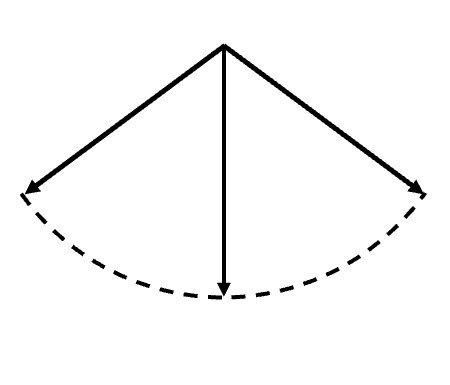
\includegraphics[width=\linewidth]{images/amplitude_wave_vectors.jpg}
		\caption{}
		\label{fig:amplitude_wave_vectors}
	\end{subfigure}
	\begin{subfigure}[t]{0.6\textwidth}
		\centering
		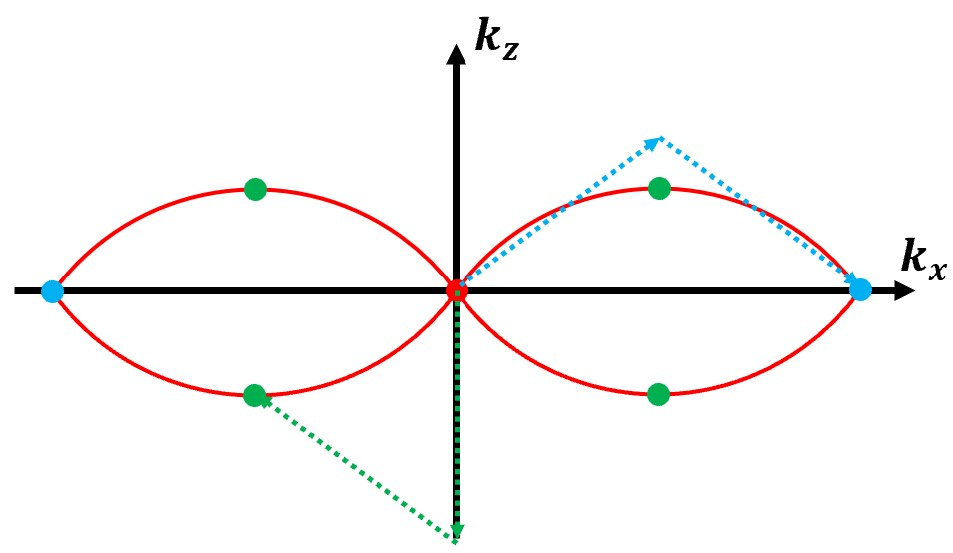
\includegraphics[width=\linewidth]{images/3D_SIM_OTF_beam_pos_w_vectors.jpg}
		\caption{}
		\label{fig:3D_SIM_OTF_beam_pos_w_vectors}
	\end{subfigure}
	
	\begin{subfigure}[t]{0.35\textwidth}
		\centering
		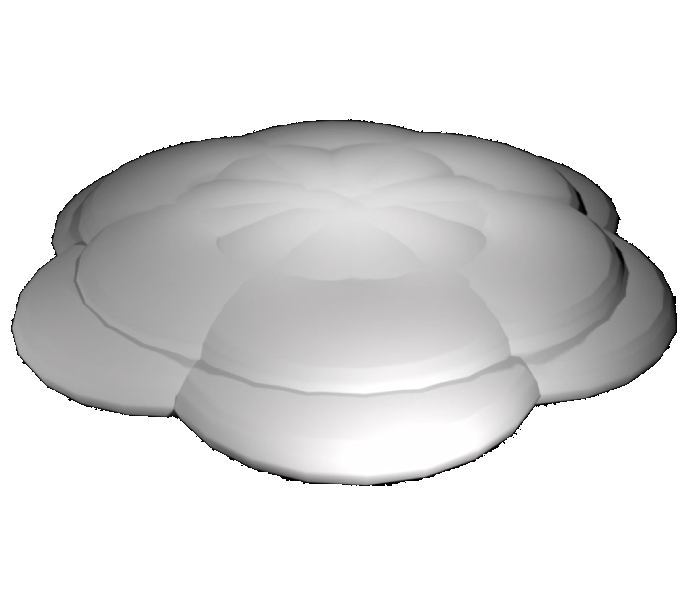
\includegraphics[width=\linewidth]{images/3D_SIM_OTF_all_angles.png}
		\caption{}
		\label{fig:3D_SIM_OTF_all_angles}
	\end{subfigure}
	\begin{subfigure}[t]{0.625\textwidth}
		\centering
		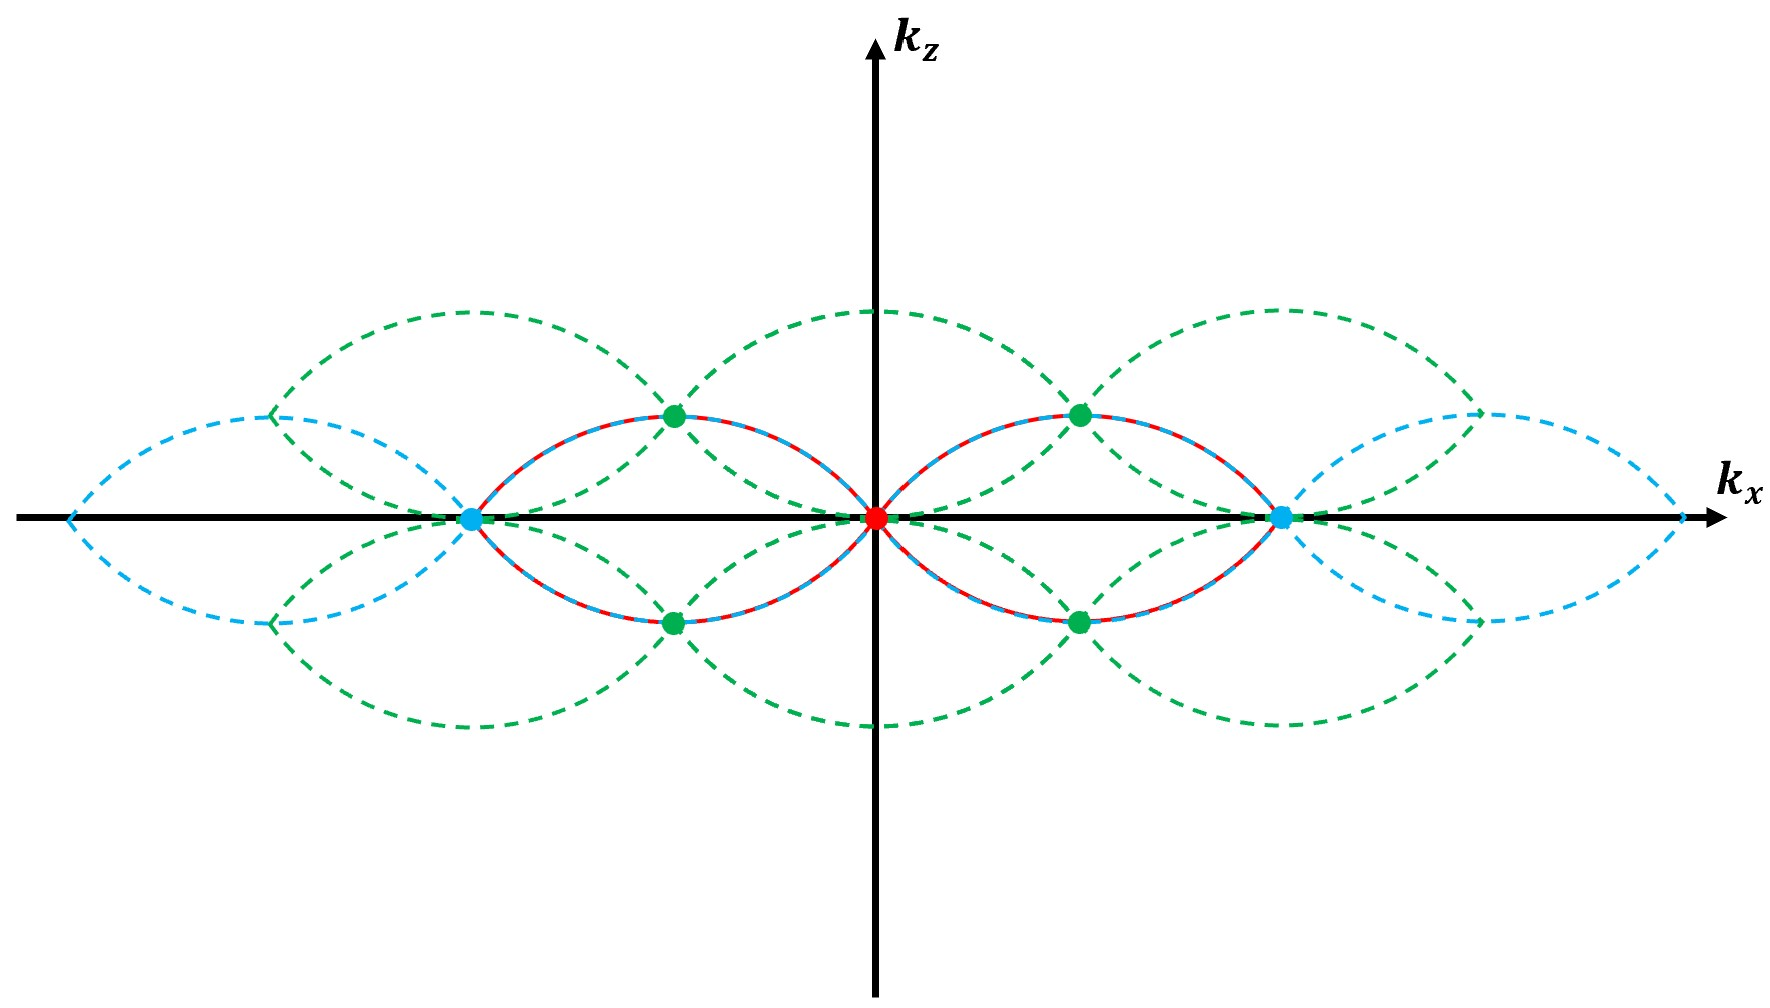
\includegraphics[width=\linewidth]{images/3D_SIM_OTF_1_angle_2D_plot.jpg}
		\caption{}
		\label{fig:3D_SIM_OTF_1_angle_2D_plot}
	\end{subfigure}	
	\caption[Resolution enhancement with 3D SIM imaging]{Resolution enhancement 
		with 3D SIM imaging. \textbf{(a)} The amplitude wave vectors 
		corresponding to the 3 illumination beams. All vectors have the 
		same magnitude, $\frac{1}{\lambda}$ \textbf{(b)} The projection of the 
		observable region onto the $k_{x}k_{z}$ plane with the spatial frequency 
		component locations for three-beam interference patterns shown. 
		\textbf{(c)} The full observable region extension for all three angles in 
		reciprocal space. \textbf{(d)} The projection of the extended observable 
		region for one stripe angle onto the $k_{x}k_{z}$ plane.}
	\label{fig:3D_SIM_visualisation}
\end{figure*}

As previously mentioned, SIM is the most widely accepted 
super-resolution technique for biology for a number of reasons. The 
number of images required in order to reconstruct a super-resolution 
SIM image, are determined by the number of lateral Fourier components 
in the illumination pattern - 3 for 2D SIM and 5 for 3D SIM - and the
number of stripe angles used to rotate the illumination pattern through
- typically 3. Therefore, only 9 or 15 images are required to 
reconstruct a 2D or 3D super-resolution SIM image respectively. This
has a number of benefits. Firstly, the temporal resolution is 
considerably higher for SIM than for point-scanning super-resolution
techniques such as STED or SMLM techniques which require a great deal more 
images per reconstruction\cite{schermelleh2019super,leung2011review}.
Secondly, each of these images is fundamentally still a widefield-style
image and therefore has a lower light-dosage than per image than STED 
or SMLM techniques. The lower light-dosage per image combined with fewer
total images required per reconstruction contributes to a low 
photodamage impact. Finally, SIM is easily expandable to multi-colour 
imaging, even using the same optical 
setup\cite{wu2018faster,allen2014structured}. Overall, SIM is a 
super-resolution technique well suited to biological imaging, 
particularly imaging dynamic biological processes.

\section{Optical Aberrations}
\label{sec:aberrations}

One factor preventing microscopes from achieving the ideal diffraction
limited resolution is the presence of optical 
aberrations\cite{goodman2005introduction,wyant1992basic,wolf1951diffraction}.
These aberrations describe the deviation of the light wavefront
from the ideal Gaussian surface. They have numerous sources, but the most
common are those arising from system imperfections - i.e. manufacturing errors
in components, placement of lenses off the optical axis, etc - and those
arising refractive index variances across the 
wavefront\cite{kubby2013adaptive,booth2007adaptive}. In biological samples, 
these variances arise from sample heterogeneities since different biological
structures possess varied refractive 
indices\cite{bashkatov2011optical, jacques2013optical, kim2010measurement, sandell2011review}.
These refractive index variances introduce path differences between 
different section of the light wavefront. A generalised pupil function 
(GPF) defined as\cite{antonello2014optimisation}:

\begin{equation}\label{eq:GPF}
P\left(\textbf{r}_{xy}\right) = A\left(\textbf{r}_{xy}\right)e^{i\Phi\left(\textbf{r}_{xy}\right)},
\end{equation}

is a complex-valued function. Defining the GPF on the normalised system 
pupil and assuming the pupil is circular simplifies the following analysis
and is generally more intuitive. In such a system, the GPF has the form:

\begin{equation}\label{eq:GPF_polar}
P\left(\rho,\theta\right) = A\left(\rho,\theta\right)e^{i\Phi\left(\rho,\theta\right)}.
\end{equation}

The real-valued function $A\left(p,\theta\right)$ accounts for amplitude
aberrations and the real-valued function $\Phi\left(p,\theta\right)$ 
accounts for the phase aberrations. Revisiting the simplified optical
system in Figure~\ref{fig:simplified_microscope_layout}, assuming a point
source a $\textbf{O}$ and that the exit pupil of the system is the unit 
disk, the field intensity at the $x'y'$ plane is proportional 
to\cite{goodman2005introduction,born2013principles}:

\begin{equation}\label{eq:image_field_insentity_GPF}
\mathcal{I}(v,\phi) = \frac{1}{\pi}\left|\int^{1}_{0}\int^{2\pi}_{0}P\left(\rho,\theta\right)e^{iv\rho\cos(\theta-\phi)}\rho d\rho d\theta\right|^{2}.
\end{equation}

For an aberration free system, $A\left(\rho,\theta\right) = 1$ and 
$\Phi\left(\rho,\theta\right) = 0$ which makes the integral in 
Equation~\ref{eq:image_field_insentity_GPF} analytically computable. From 
this it is possible to recover $\mathcal{I}(v,\phi) = \mathcal{I}_{w}(v)$
from Equation~\ref{eq:image_field_insentity}.

\subsection{Zernike Polynomials}
\label{subsec:zernike}

Whilst the phase distortions can be treated in their native form, it is 
useful for a number of reasons to represent them as an expansion in
orthogonal functions, and Zernike polynomials are typically chosen for 
this expasion\cite{zernike1934diffraction,noll1976zernike,mahajan1994zernike}.
Zernike modes are not suitable to represent phase distortions arising 
from all sources, such as air turbulence or fabrication errors in the 
single-point diamond turning process\cite{wyant1992basic}. However, the 
sources of phase distortions for which a Zernike representation is not
appropriate do not generally arise. Additionally, the Zernike modes have 
a number of useful mathematical properties, and low order Zernike modes 
correspond to well-known optical aberrations e.g. defocus, astigmatism, 
coma, spherical 
aberration\cite{born2013principles,booth2007adaptive,zernike1934diffraction}.
Using the Zernike polynomials, the phase distortions, $\Phi\left(\rho,\theta\right)$
can be written as:

\begin{equation}\label{eq:phase_zernike_expansion}
\Phi\left(\rho,\theta\right) = \sum\limits_{n,m}\alpha^{m}_{n}\mathcal{Z}^{m}_{n}\left(\rho,\theta\right),
\end{equation}

where indices $n \in \mathbb{N}_{0}$ and $m \in \mathbb{Z}$ denote the radial order 
and azimuthal frequency respectively of the Zernike polynomial, 
$\mathcal{Z}^{m}_{n}$, and are such that $n - \left|m\right| \ge 0$ and even. The
coefficients of each Zernike polynomial are represented by $\alpha^{m}_{n} \in 
\mathbb{R}$. Each Zernike polynomial is the product of a radial polynomial,
$R^{m}_{n}(\rho)$, and an azimuthal polynomial, $\Theta^{m}_{n}(\theta)$:

\begin{equation}\label{eq:zernike_polynomial}
\mathcal{Z}^{m}_{n}\left(\rho,\theta\right) = c^{m}_{n}R^{m}_{n}(\rho)\Theta^{m}_{n}(\theta),
\end{equation}

where $c^{m}_{n}$, $R^{m}_{n}(\rho)$, and $\Theta^{m}_{n}(\theta)$ have the following definitions:

\begin{equation}\label{eq:zernike_polynomial_c}
c^{m}_{n} = 
\begin{cases}
\sqrt{n + 1} & m = 0\\
\sqrt{2(n + 1)} & m \ne 0\\
\end{cases},
\end{equation}

\begin{equation}\label{eq:zernike_polynomial_R}
R^{m}_{n}(\rho) = \sum_{s=0}^{\frac{n-m}{2}}{\frac{(-1)^{s}(n-s)!}{s!\left(\frac{n+m}{2}-s\right)!\left(\frac{n-m}{2}-s\right)!}\rho^{n-2s}},
\end{equation}

\begin{equation}\label{eq:zernike_polynomial_Theta}
\Theta^{m}_{n}(\theta) =
\begin{cases}
\cos(m\theta) & m \ge 0\\
-\sin(m\theta) & m < 0\\
\end{cases}.
\end{equation}

This formulation of Zernike modes is normalised and ordered according
to the Noll indexing convention, although other modal bases and ordering 
conventions do exist\cite{noll1976zernike,thibos2002standards,
	loomis1978computer,soloviev2017optimal,burton1984effects}. 

It is useful to be able to compare phase distortions to one another to
measure their severity. In order to do so, scalar indicators are required.
Typically, the root mean squared (rms) and variance of $\Phi\left(\rho,\theta\right)$
are used:

\begin{align}\label{eq:scalar_indicators}
rms(\Phi) = \left(E_{2}\left[\Phi\right]\right)^{\frac{1}{2}} && 
var(\Phi) = E_{2}\left[\Phi\right] - \left(E_{1}\left[\Phi\right]\right)^{2},
\end{align}

where $E_{k}\left[\Phi\right]$ are the 
functionals\cite{antonello2014optimisation,mahajan1994zernike}:

\begin{equation}\label{eq:E_functionals}
E_{k}\left[\Phi\right] = \frac{1}{\pi} \int_{0}^{1}\int_{0}^{2\pi} \Phi\left(\rho,\theta\right)^{k}\rho d\rho d\theta.
\end{equation}

Using the normalisation factors, $c_{n}^{m}$, and the orthogonality
properties of the Zernike modes, it is apparent that $E_{1}\left[\Phi\right] 
= \alpha_{0}^{0}$ and $E_{2}\left[\Phi\right] = 
\sum\limits_{n,m}{\left({\alpha_{n}^{m}}\right)^{2}}$. Substituting 
these values back into Equations~\ref{eq:scalar_indicators} yields:

\begin{align}\label{eq:scalar_indicators_new}
rms(\Phi) = \left(\sum\limits_{n,m}{\left({\alpha_{n}^{m}}\right)^{2}}\right)^{\frac{1}{2}} && 
var(\Phi) = \sum\limits_{n\ne 0,m\ne 0}{\left({\alpha_{n}^{m}}\right)^{2}},
\end{align}

Since $\mathcal{Z}_{n}^{m}$  (XX shouldnt this be n=0, m=0? XX)- i.e. piston - does not affect image 
formation, often its corresponding amplitude $\alpha_{0}^{0}$ is
simply not included. In this case, $rms(\Phi) = \sqrt{var(\Phi)}$

\subsection{Aberrations and Resolution}
\label{subsec:aberrations_and_resolution}

Not all Zernike modes affect the resolution of the system. 
Figures~\ref{fig:Airy_ring_2D_2_object_seperation_aberration_comparison_Noll_1}-
\ref{fig:Airy_ring_2D_2_object_seperation_aberration_comparison_Noll_3}
show the effect of the first 3 Zernike modes, $\mathcal{Z}_{0}^{0}$, 
$\mathcal{Z}_{1}^{-1}$, and $\mathcal{Z}_{1}^{1}$ - i.e. piston, tip and 
tilt - on two point objects separated by the diffraction limit determined
by the Rayleigh criterion, $r_{l}$. Clearly piston has no effect on the 
image intensity or resolving power. Additionally, assuming an incoherent, 
shift invariant imaging system, the only effect of the tip and tilt 
aberrations is a lateral shift in the $x$ and $y$ axis respectively. The
overall image intensity and resolving power remains unaffected. For this 
reason piston (and often tip and tilt) are considered ``non-optical'' 
aberrations. 
Figure~\ref{fig:Airy_ring_2D_2_object_seperation_aberration_comparison_rms_1}
shows the same two point objects aberrated with phase deformations of 
$rms(\Phi) = 1$. The image intensity is severely degraded and the resolving
power is significantly less than the diffraction limited case. Evidently, 
the presence of phase distortions is a limiting factor to imaging systems 
from achieving the ideal diffraction limited 
resolution\cite{antonello2014optimisation,booth2014adaptive}.

\begin{figure*}
	\centering
	\begin{subfigure}{0.49\textwidth}
		\centering
		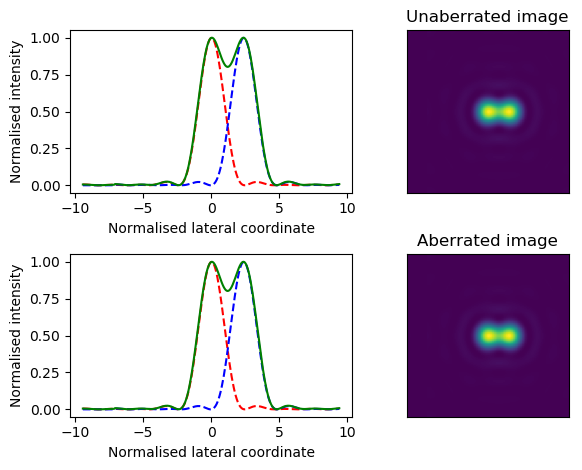
\includegraphics[width=\linewidth]{images/Airy_ring_2D_2_object_seperation_aberration_comparison_Noll_1.png}
		\caption{$rms(\Phi) = 1, \alpha_{0}^{0} = 1$}
		\label{fig:Airy_ring_2D_2_object_seperation_aberration_comparison_Noll_1}
	\end{subfigure}
	\begin{subfigure}{0.49\textwidth}
		\centering
		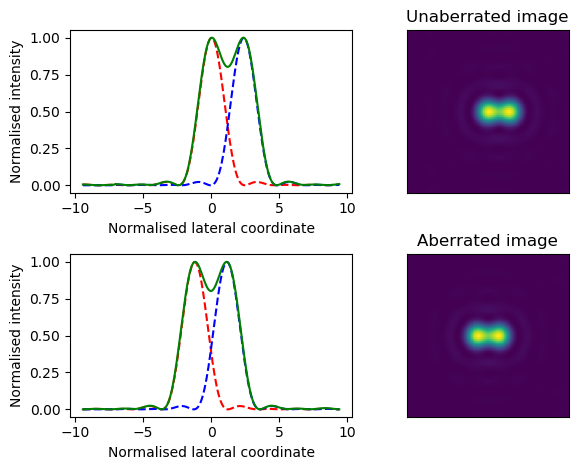
\includegraphics[width=\linewidth]{images/Airy_ring_2D_2_object_seperation_aberration_comparison_Noll_2.png}
		\caption{$rms(\Phi) = 1, \alpha_{1}^{-1} = 1$}
		\label{fig:Airy_ring_2D_2_object_seperation_aberration_comparison_Noll_2}
	\end{subfigure}
	\begin{subfigure}{0.49\textwidth}
		\centering
		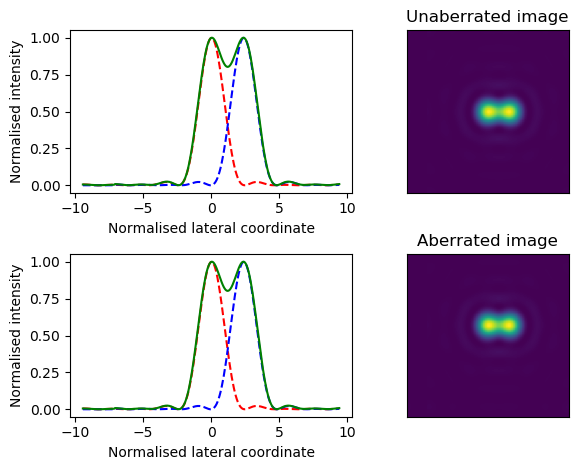
\includegraphics[width=\linewidth]{images/Airy_ring_2D_2_object_seperation_aberration_comparison_Noll_3.png}
		\caption{$rms(\Phi) = 1, \alpha_{1}^{1} = 1$}
		\label{fig:Airy_ring_2D_2_object_seperation_aberration_comparison_Noll_3}
	\end{subfigure}
	\begin{subfigure}{0.49\textwidth}
		\centering
		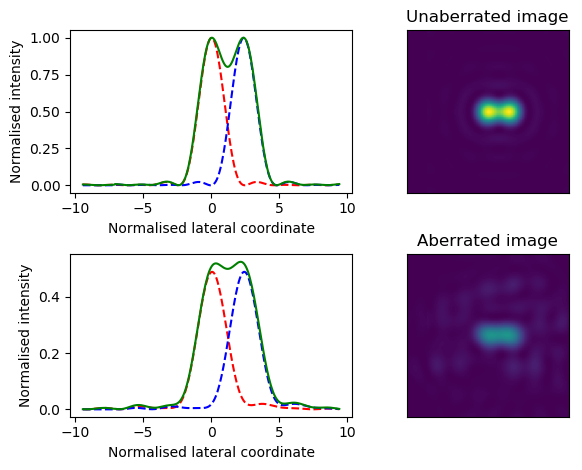
\includegraphics[width=\linewidth]{images/Airy_ring_2D_2_object_seperation_aberration_comparison_rms_1.png}
		\caption{$rms(\Phi) = 1$}
		\label{fig:Airy_ring_2D_2_object_seperation_aberration_comparison_rms_1}
	\end{subfigure}
	\caption[A visualisation of the effect of optical aberrations on image 
	resolution]{A visualisation of the effect of optical aberrations on 
		image resolution \textbf{(a)-(c)} Ideal diffraction limited point 
		sources at separation $r_{l}$ aberrated with $rms(\Phi) = 1$ of purely 
		piston, tip, and tilt respectively. \textbf{(d)} Ideal diffraction 
		limited point sources at separation $r_{l}$ aberrated with a random 
		phase distortion with $rms(\Phi) = 1$}
	\label{fig:aberrations_res}
\end{figure*}

\section{Adaptive Optics}
\label{sec:AO}

As previously mentioned, phase aberrations arise in microscopy primarily
due to heterogeneities in the structure of the biological sample being 
imaged. Consider the objective lens of a microscope, in the absence of
optical aberrations, as in Figure~\ref{fig:wavefront_focus_ideal}, a flat
wavefront is focused to a single diffraction limited spot. Introducing
a heterogeneous media distorts the phase wavefront and leads to an 
extended, non-diffraction limited focal spot as seen in 
Figure~\ref{fig:wavefront_focus_aberrated}. However, if, as in 
Figure~\ref{fig:wavefront_focus_corrected} the wavefront is not flat when 
it enters the microscope objective but instead shaped to compensate for 
the phase distortion, then an ideal, diffraction limited focal spot is 
recovered. Since the phase distortions encountered are not only sample
dependent, but spatially and (for live samples) temporally dependent an
adaptive method for pre-shaping the optical wavefront is 
required\cite{schwertner2004characterizing,wang2014multiplexed,girkin2009adaptive}.
The branch of technologies and methods for doing this is referred to as
adaptive optics (AO).

\begin{figure}[h]
	\centering
	\begin{subfigure}[t]{0.3\textwidth}
		\centering
		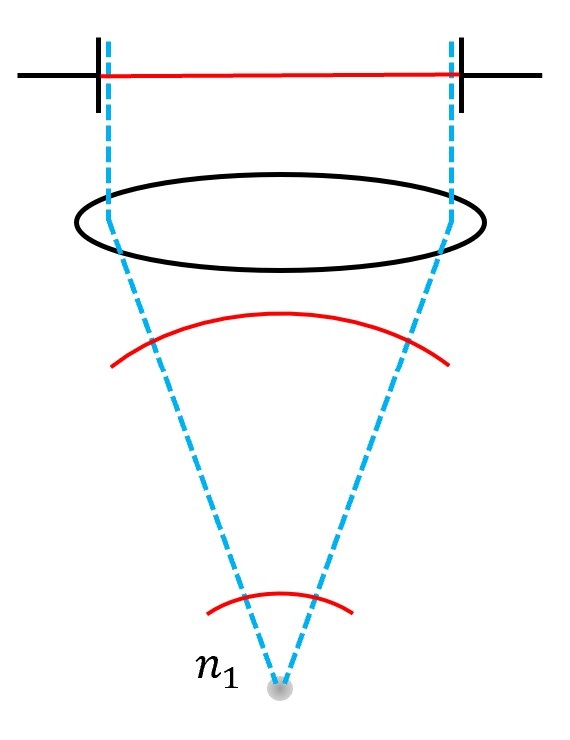
\includegraphics[width=\linewidth]{images/wavefront_focus_ideal.jpg}
		\caption{}
		\label{fig:wavefront_focus_ideal}
	\end{subfigure}
	\begin{subfigure}[t]{0.3\textwidth}
		\centering
		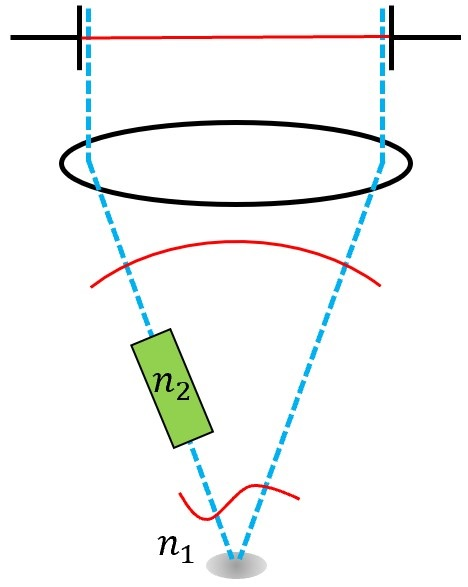
\includegraphics[width=\linewidth]{images/wavefront_focus_aberrated.jpg}
		\caption{}
		\label{fig:wavefront_focus_aberrated}
	\end{subfigure}
	\begin{subfigure}[t]{0.3\textwidth}
		\centering
		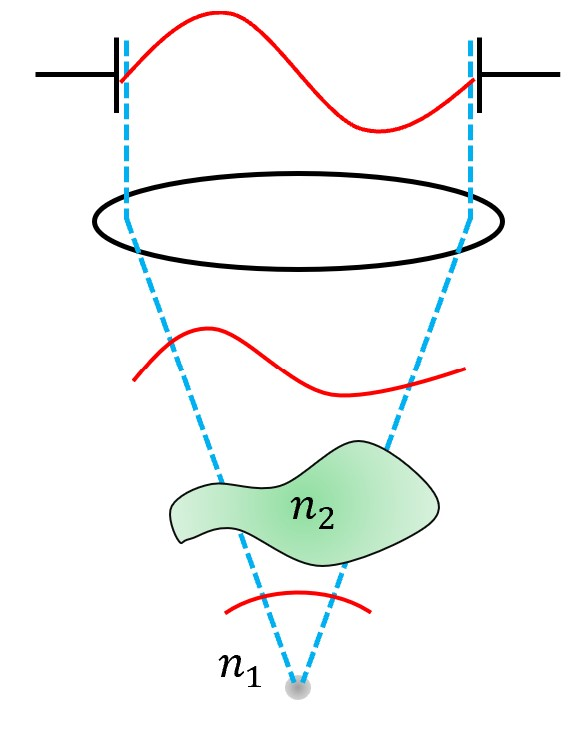
\includegraphics[width=\linewidth]{images/wavefront_focus_corrected.jpg}
		\caption{}
		\label{fig:wavefront_focus_corrected}
	\end{subfigure}
	\caption[Illustration of aberrations affecting a microscope
          objective focus.]{Illustration of aberrations affecting a
          microscope objective focus. \textbf{(a)} The media between
          the microscope objective and the sample has a homogeneous refractive index, $n_{1}$ and the microscope objective forms a diffraction limited focal spot. \textbf{(b)} the media the wavefront passes through is heterogeneous. This causes a phase distortion in the wavefront and leads to an expanded focal spot. \textbf{(c)} Prior to the objective aperture, the wavefront is pre-shaped to the opposite shape to the expected distortion. Once the wavefront passes though the heterogeneous media, an ideal wavefront is recovered and thus the focal spot is diffraction limited again.}
	\label{fig:wavefront_focus}
\end{figure}

Similar to how the telescope and microscope have a shared historical origin,
the concept of using AO to correct for optical aberrations has it is 
origin in correcting for phase distortions in astronomical telescopes\cite{babcock1990adaptive}.
The principle of an AO system for microscopy is shown in 
Figure~\ref{fig:ao_system_schematic_simple}. Here, only the emission path 
is considered. A distorted wavefront $\Phi_{I}$, arrives at the aperture 
of the microscope. The wavefront is then imaged onto an adaptive element 
capable of applying a variable phase distortion, $\Phi_{AO}$. Once the 
wavefront has interacted with the adaptive element, there is a residual 
phase aberration $\Phi_{R} = \Phi_{I} - \Phi_{AO}$. 
Figure~\ref{fig:ao_system_schematic_simple} has the wavefront passing through
a beamsplitter and both being focused onto an imaging device and being 
directed to a wavefront sensor. In the latter case, $\Phi_{R}$ is 
calculated directly while in the former case $\Phi_{R}$ is inferred through 
some indirect measurement. Typically only one of these options is employed. 
The calculation of $\Phi_{R}$ is then passed to a controller which adjusts 
$\Phi_{AO}$ in order to minimise some measure of error such as $rms(\Phi_{R})$. 
Figure~\ref{fig:ao_system_schematic_simple} assumes a reflective adaptive 
element such as a deformable mirror (DM) or a spatial light modulator (SLM), 
but the principles also apply for a transmissive adaptive element placed 
in the beam path, such as an opto-acoustic lens.

\begin{figure}[h]
	\centering
	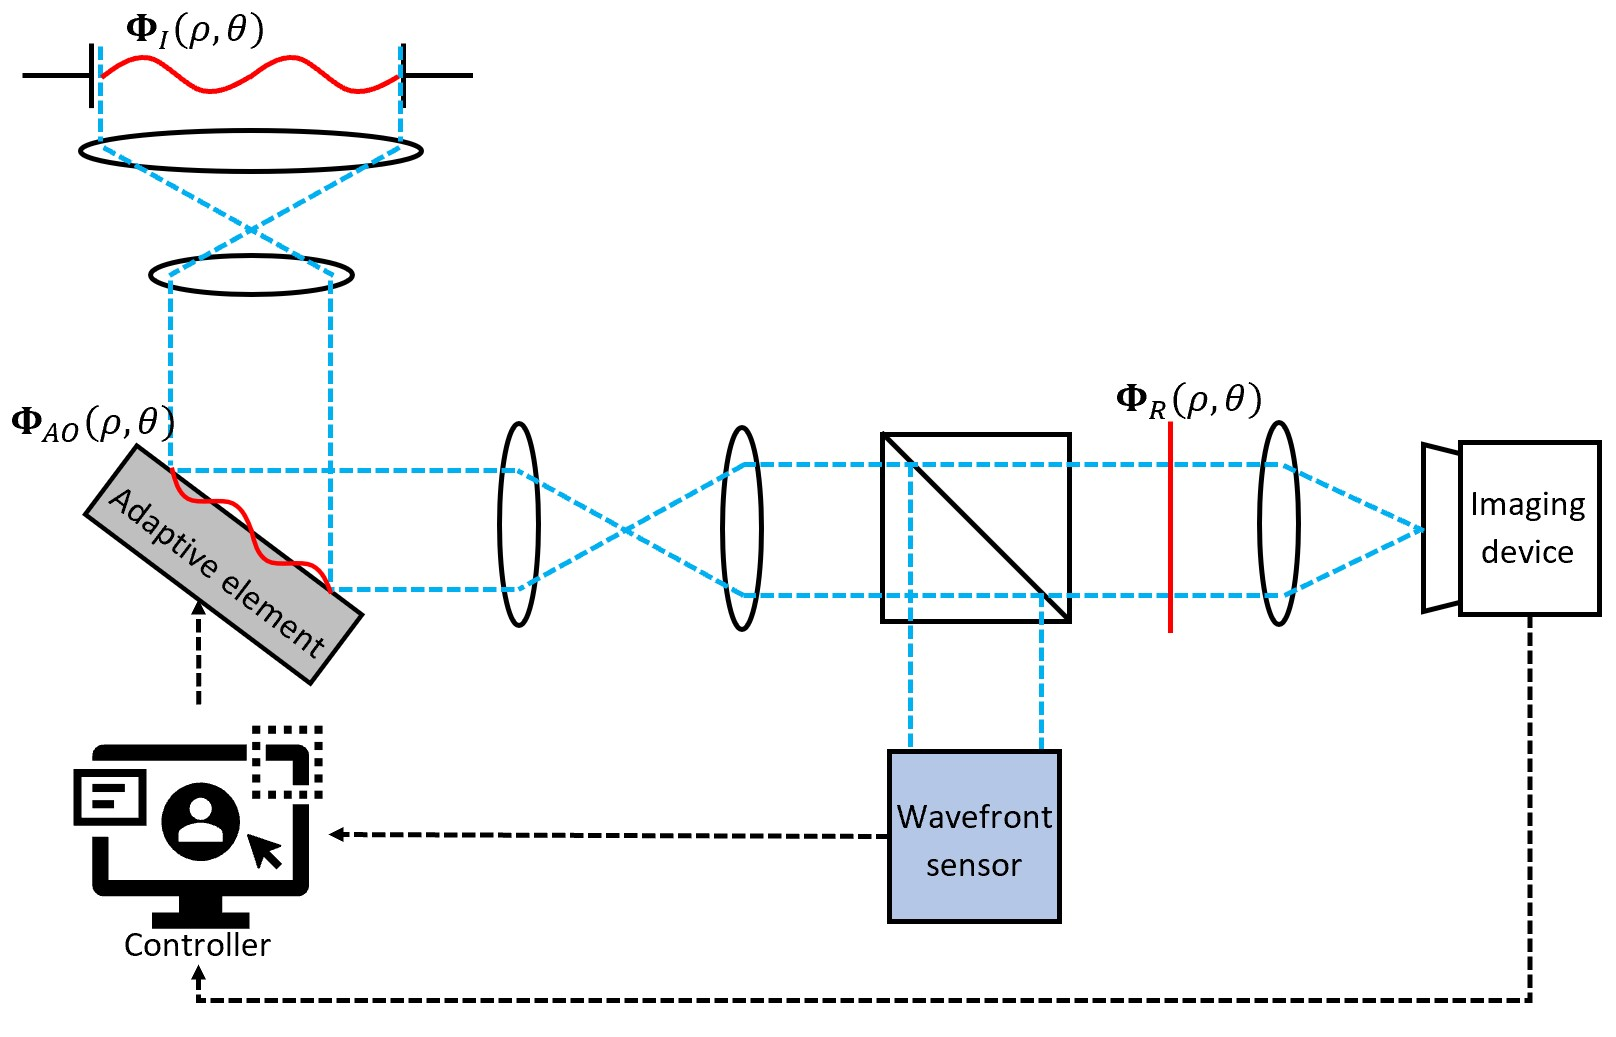
\includegraphics[width=\textwidth]{images/ao_system_schematic_simple.jpg}
	\caption[Schematic of the emission path of an adaptive optics
          system.]{Schematic of the emission path of an adaptive
          optics system. The emitted wavefront of a point in the
          fluorescent sample, $\Phi_{I}$, arrives at the aperture of
          the microscope. It is reimaged onto the adaptive
          element. The adaptive element has some phase, $\Phi_{AO}$,
          on its surface. The light then passed through a beamsplitter
          and is focused onto an imaging device. The residual phase
          aberration, $\Phi_{R} = \Phi_{I} - \Phi_{AO}$, is either
          calculated directly by the wavefront sensor or inferred
          indirectly from the data acquired by the imaging
          device. This information is passed to a controller which
          applies a phase aberration to the adaptive element,
          $\Phi_{AO}$, in order to minimise a metric like $rms(\Phi_{R})$.}
	\label{fig:ao_system_schematic_simple}
\end{figure}

Implementing AO in microscopy has already been shown to be highly 
effective at reducing optical aberrations and yielding significant 
improvements to image 
quality\cite{booth2014adaptive,girkin2009adaptive,fraisier2015adaptive,jesacher2011sensorless,
	jian2014wavefront}. Designing an AO enabled system follows a predicable 
workflow outlined in Figure~\ref{fig:ao_system_setup_workflow} 
consisting of four phases:

\begin{enumerate}
	\item \textit{System Design Phase}: A potential user should consider 
	the needs of their imaging modality, system constraints, desired 
	sample types before deciding on the appropriate AO element to 
	implement.
	\item \textit{Installation Phase}: The user installs the chosen AO 
	element into their beam path.
	\item \textit{Set-up Phase}: The AO element is calibrated to correct 
	for optical aberrations. This calibration is checked and the system 
	aberrations are corrected.
	\item \textit{Sample Correction Phase}: The sample correction routine 
	is designed. This will typically fall into one of two categories; 
	sensorless AO or direct wavefront sensing.
\end{enumerate}  

However, there are a number of adaptive elements\cite{olivier2002advanced}, 
a plethora of direct wavefront sensing techniques\cite{antonello2014optimisation,trumper2016instantaneous,
	schwertner2004measurement}, and wide array of 
sensorless correction methodologies\cite{burke2015adaptive,booth2002adaptive,
	fienup2003aberration,antonello2020multi,debarre2007image}. 
Considering AO within super-resolution imaging techniques further complicates
the 
situation\cite{debarre2008adaptive,booth2015aberrations,thomas2015enhanced}.
Since there is no universally agreed upon AO implementation, each 
implementation has to go through the entire design process from scratch, 
creating a bespoke but brittle implementation which is not easily transferable
to any other system, imaging modality, sample type, etc. 

\begin{figure}[h]
	\centering
	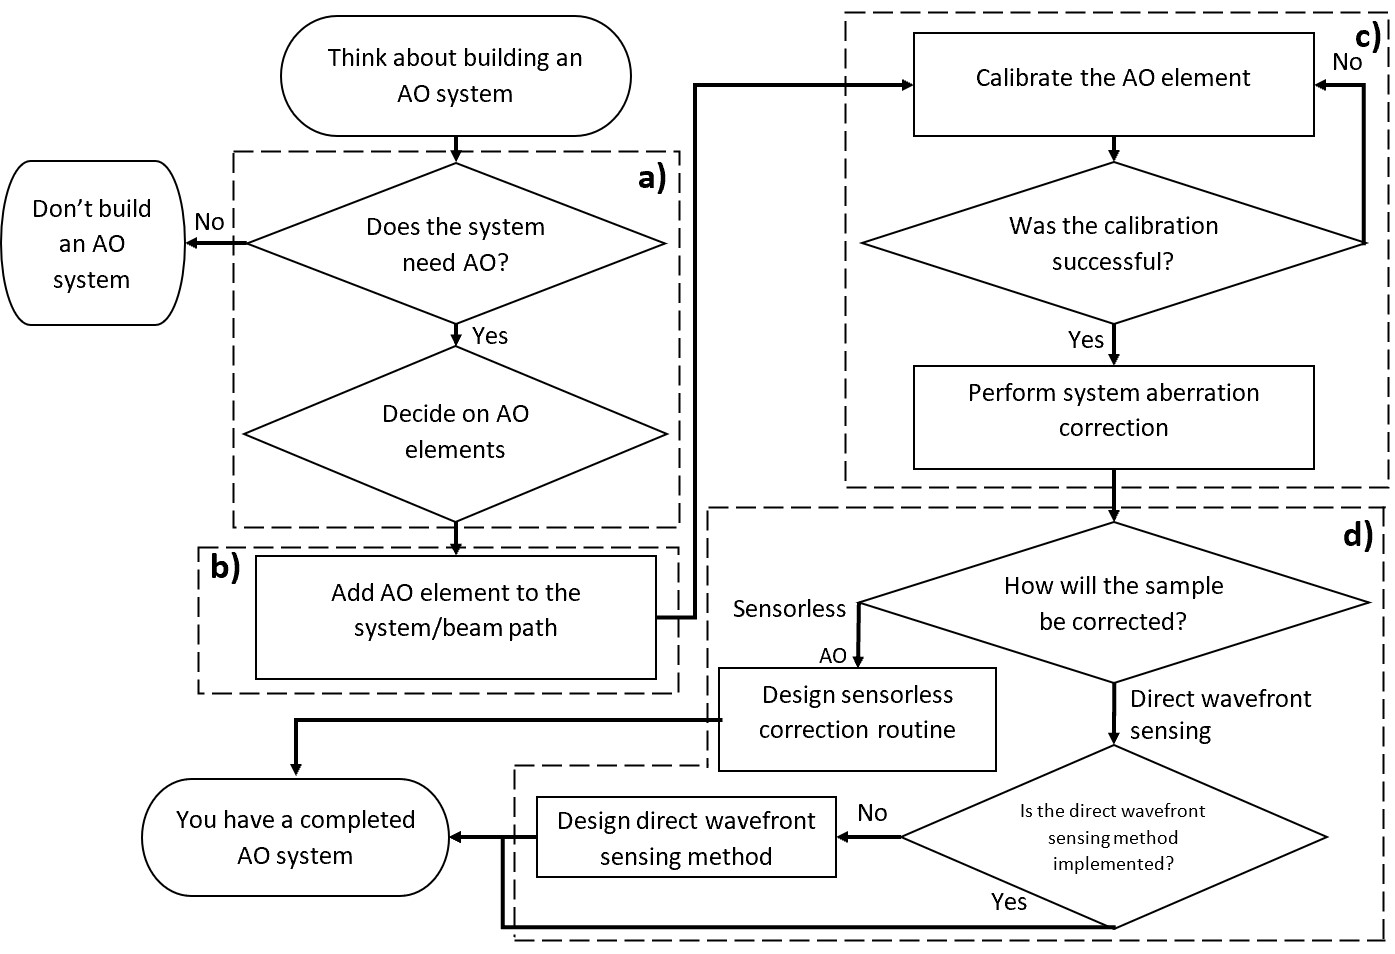
\includegraphics[width=1\textwidth, scale=0.5]{./images/ao_system_setup_workflow_new.jpg}
	\caption[Flowchart depicting the general process for building a system utilising AO.]{Flowchart depicting the general process for building a system utilising AO. \textbf{a)} \textit{System Design Phase}. User decides whether the system needs AO and, if so, what type. \textbf{b)} \textit{Installation Phase}. The chosen AO elements are added to the system. \textbf{c)} \textit{Set-up Phase}. The chosen AO element is calibrated. Typically, this involves mapping the variable elements of the AO element (e.g. deformable mirror actuators) to a useful set of basis functions which represent optical aberrations. \textbf{d)} \textit{Sample Correction Phase}. Here the user designs the methods to be used for correcting their desired sample.}
	\label{fig:ao_system_setup_workflow}
\end{figure}

\section{Overview and Aims of the Thesis}
\label{sec:overview}

There is a need for a robust, accurate, easy-to-use, general implementation 
of AO for microscopy\cite{ji2017adaptive,rodriguez2018adaptive}.
This implementation should be accessible to users in order to ensure its
adoption amongst the microscopy community and therefore the widespread 
adoption of AO technology. This thesis demonstrates just such an 
implementation - Microscope-AOtools - deployed successfully on two separate 
systems. The contributions of the thesis are collected into four chapters 
and is laid out as follows:

\begin{itemize}
	\item Chapter 2 discusses the two systems which Microscope-AOtools has
	been deployed on: Aurox Clarity and DeepSIM. It discusses their optical 
	layout and contains a brief discussion of the optical alignment 
	procedure as well as an alignment tool developed during the course of 
	this thesis; ``Hall, Nicholas J., David Miguel Susano Pinto, and Ian M. 
	Dobbie. "BeamDelta: simple alignment tool for optical systems." 
	\textit{Wellcome Open Research} 4.194 (2019): 194.''\cite{dobbie2019beamdelta} 
	The hardware control software - Python Microscope - used to synchronise 
	the disparate hardware elements of each microscope setup and the 
	graphical user interface (GUI) software - Microscope-Cockpit - which 
	is used to operate the microscopes are also discussed.
	\item Chapter 3 corresponds to scientific publication: ``Hall, Nicholas, 
	et al. ``Microscope-AOtools: A generalised adaptive optics 
	implementation.''
	\textit{Optics Express} 28.20 (2020): 28987-29003.''\cite{hall2020microscope}
	The generalised implentations of all the methods required by the Set-up and 
	Sample Correction phases detailed in Section~\ref{sec:AO} are discussed.
	It also contains discussion of the integration of Microscope-AOtools with
	Microscope-Cockpit in order to enable accessibility for users.
	\item Chapter 4 corresponds to the scientific publication: ``Hussain, 
	Syed Asad, et al. ``Wavefront-sensorless adaptive optics with a 
	laser-free spinning disk confocal microscope.'' \textit{Journal of 
		Microscopy} (2020).'' 
	on which the author is a co-first author\cite{hussain2020wavefront}. It details the successful 
	implementation of Microscope-AOtools on the Aurox Clarity system.
	\item Chapter 5 details the successful implementation of Microscope-AOtools 
	on the DeepSIM system. The results and implementation presented here will
	contribute significantly to a future publication of the DeepSIM system.
\end{itemize}

Discussions of existing limitations and areas for further development to the 
presented AO implementation are presented in Chapter 6. Conclusions are drawn 
in Chapter 7. The Aurox Clarity system was built by Dr Syed Hussain of the 
Dynamic Optics and Photonics Group, University of Oxford and Toshiki Kubo
Department of Applied Physics, Osaka University. The design and original 
implementation of the DeepSIM system was built by Dr Ian Dobbie, Dr Mick 
Philips, Dr Antonia G\"{o}hler and Dr Mantas \v{Z}urauskas, 
all members of the Micron Advanced Imaging Consortium at the time. The author 
implemented a number of modifications, improvements, and realignments in 
order to produce the demonstrations shown in this thesis.
